\documentclass[12pt]{thesis} %%%%%%%%%%%%%%%%%%%%%%%%%%%%%%%%%%%%%%%%%%%%%%%%%%
\usepackage[utf8]{inputenc}

\newcommand{\autor}{Nils Heine} % Vor und Nachname / GivenName FamilyName (The one on your matriculation)
\newcommand{\matrikel}{6703759}	% Matrikel / Matriculation number
\newcommand{\erstgutachter}{Prof. Dr.-Ing. Timo Gerkmann} % Erstgutachter / Primary Reviewer
\newcommand{\zweitgutachter}{Dr.-Ing. Martin Krawczyk-Becker} % Zweitgutachter / Secondary Reviewer
%\newcommand{\betreuer}{Name Betreuer} % Betreuer  delete / comment this line if you didn't have a supervisor or the supervior is one of the reviewers
\newcommand{\arbeitstitel}{Real-Time Automatic Gain Control for Singing Voice Applications} % Titel angeben / title of your thesis
\newcommand{\arbeitstyp}{Bachelor Thesis} %Typ angeben / type of the thesis 
\newcommand{\studycourse}{Informatik} % Studiengang/ study course

\usepackage{hcisty}

\usepackage{todonotes}
\usepackage{amsmath}
\usepackage{algorithm}
\usepackage[noend]{algpseudocode}
\usepackage{booktabs}

\newcommand\tab[1][1cm]{\hspace*{#1}}


% WORDS THAT SHOULD NOT BE HYPHENATED (am seitenende nicht geteilt?!)
\hyphenation{DAW}


\start{1}{1}
% \start[1]{1} <= show both abstracts
% \start[0]{1} only german. \start[1]{0} only english .\start[0]{0} nothing
% change the abstract.tex and abstractGER.tex to your needs
\newpage\chapter{Introduction}
\label{chapter:introduction}




\newpage\chapter{Basics}
\label{chapter:basics}

\section{Loudness}

Including the human perception in the algorithm is a complex task as for example absolute threshold of hearing and the subjective perception of sound pressure are varying for different frequencies (see Fig. \ref{LDNSGraph}).\\

\begin{figure}[H]
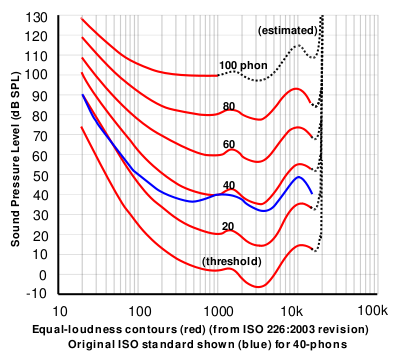
\includegraphics[width=0.5\textwidth]{images/loudnessGraph}
	\centering
	\caption{Loudness perception\cite{wikiLoud}}
	\label{LDNSGraph}
\end{figure}

While gathering information on how to improve the plug-in in terms of human perception the ITU-R BS.1770-4\cite{ITUalgo} algorithm was evaluated. This algorithm classifies an audio file for its humanly perceived loudness. It is mainly used by television and music streaming services as the program loudness can be kept steady while switching content. As the perception is of substantial interest for mixing a song, this was investigated in this study. Due to a good documentation about how to implement the loudness algorithm a copy of it was build in Python and it was decided which elements to be adopted in the plug-in. The first and second element were two filters. Their use is to mimic the human perception of sound pressure at different frequencies. The first filter is a low cut for the reason that human hearing is insensitive to low frequencies. The second filter is a high shelf and is ‘\textit{used to account for the acoustic effects of the head}’\cite{ITUalgo}. This imitation of the human hearing is substantially simplified but cost-effective in terms of computation. The low cut filter has a cutoff frequency of 38 Hz, the high shelf of around 1681 Hz.\\

\begin{figure}[H]
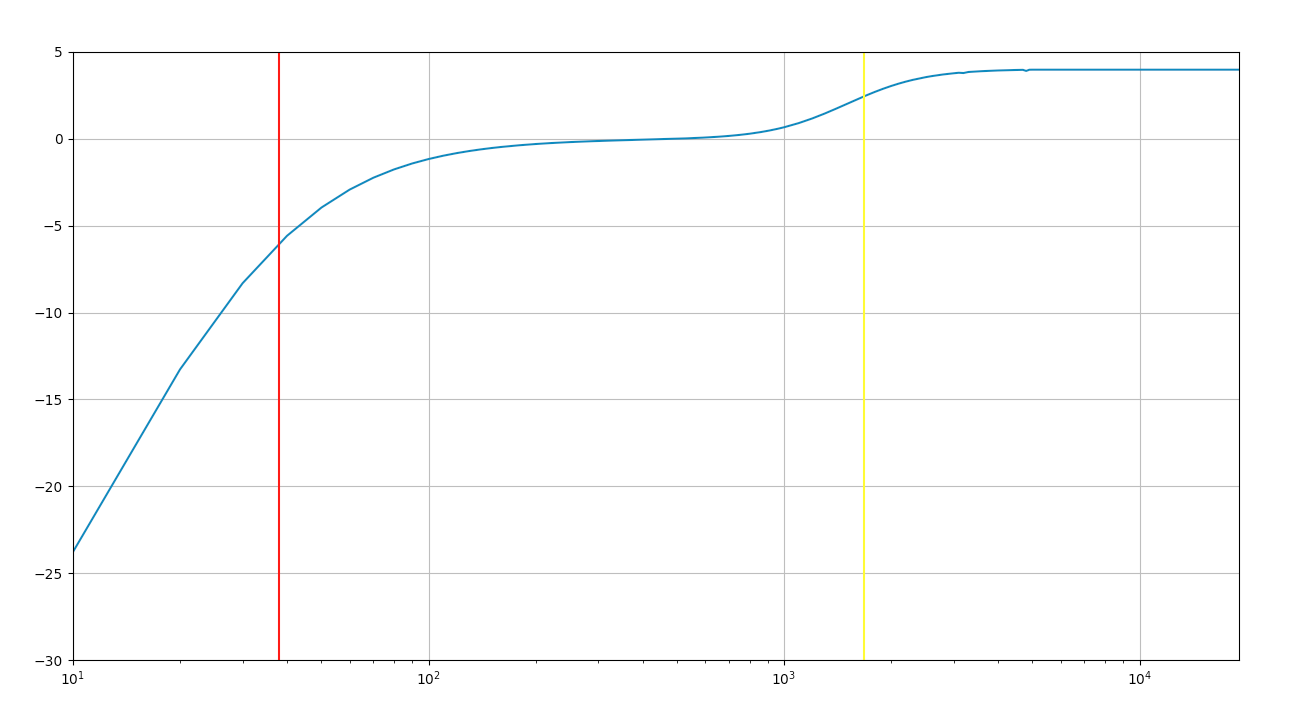
\includegraphics[width=0.8\textwidth]{images/filter_test}
	\centering
	\caption{Plotted outcome of adopted filter implementation for the audible spectrum of frequencies}
	\label{filterTest}
\end{figure}

The filter section is followed by the determination of a root mean square (RMS) value for time windows of 400ms overlaping 75\% (a value is saved every 100ms). This means it is calculating the root of the average from the squares of each sample in the set time window which equals the power of the signal.\\
RMS calculation is used because it is part of the imitation of human perception: a human will not interpret a small impulse of a handful of samples as loud as a audio signal at the same level of longer duration.  For example ‘\textit{a 3-msec pulse must have a level about 15 dB higher to sound as loud as a 0.5-sec (500-msec) pulse}'\cite{masterHA}.\\
Subsequently, all RMS values below a absolute threshold of -70LKFS\footnote{definition in \cite{ITUalgo}} are sorted out by a gate and a average value is determined. Another gate of -10LU below the average is applied on the rms values and a second averaging of measurements is performed. The resulting average is the loudness of the processed audio file.\\

\section{Vocal Rider}

'Vocal Rider' by Waves is a commercially available audio plug-in which realizes a automatic gain adaption for vocal signals.

\begin{figure}[H]
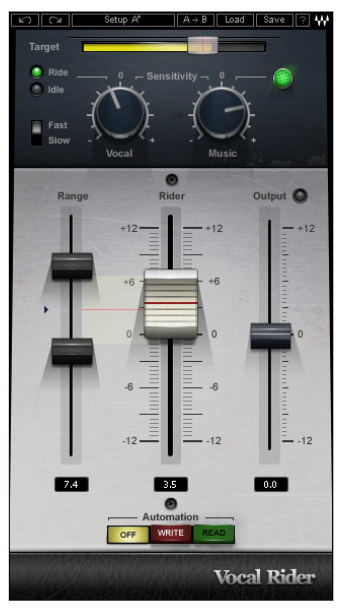
\includegraphics[width=0.35\textwidth]{images/vocalRiderUI}
	\centering
	\caption{UI of Waves 'Vocal Rider'\cite{vocalRiderM}}
	\label{VRUI}
\end{figure}

The vocal signal's level is adjusted to the set \textit{target} value (at top of Fig. \ref{VRUI}). The '\textit{target sets the reference range for vocal mix positioning. [It] (…) will move the Rider Fader’s ‘0’ calibration.}'\cite{vocalRiderM}. Additionally a user can control the maximal gain adaption with the '\textit{range}' slider and adjust the resulting level to the backtrack via a output gain. For results depending on the instrumental backtrack a side chain input can be used and adjusted with the '\textit{music}' potentiometer.\\
As in this study the same basic idea is realized with a independent approach it is possible to adopt useful results from the comparison (see chapter \ref{chapter:comparison}) of both plug-ins and remain with potential advantages.\\

\section{Optimization}

For the comparison in chapter \ref{chapter:comparison} optimization methods were used to find parameters for the study plug-in to get to similar results as the 'Vocal Rider' does. Therefore the scipy\cite{scipy} methods scipy.optimize.brute and scipy.optimize.minimize were used.\\
Previously a function had to be written which returns the current problem as a number. Thereby a smaller number equals a smaller problem.\\
The '\textit{brute}' optimization algorithm '\textit{computes the function’s value at each point of a multidimensional grid of points, to find the global minimum of the function}'\cite{scipyB}. The according '\textit{grid}' is therefore previously defined for the current optimization problem. This is done by initializing a set of user defined bounds and step sizes for each of the parameters which a transferred to the function to be optimized.\\
The '\textit{minimize}' optimization algorithm per default '\textit{uses the L-BFGS-B algorithm ... for bound constrained minimization}'\cite{scipyM}. This algorithm is able to compute faster and more selective but needs a good inital parameter guess to get to a proper result.\\


\newpage\chapter{Prototype}
\label{chapter:prototype}

\section{Overview}

The basic approach works in five steps: filter, root mean square (RMS) calculation, gate, gain adaption, delay.\\
The processing chain starts with a low-cut and a high-shelf filter which will be applied sample wise on the incoming audio. These filters are a simplified mapping of the perception of sound pressure for human beings. This is the first step to adjust the plug-in to loudness instead of sound pressure (as done in FOOTNTE). However, the plug-in won’t be running with the full loudness detection algorithm (FUTNOT) due to calculation time and real time capability (see SPÄTER? oder hier?).\\
After the filter section every sample is passed to the RMS calculation.  The goal is to output the squared average of a previously specified period of time. The square root will be determined in the following calculation of the equivalent dB value. The plug-in converts the linear audio samples into the logarithmic dB scale in order to display gain values and loudness goal (see gain part?) in dB in the user interface (UI) as it is the standard scale of DAWs. Thereby the executive sound engineer will intuitively know how to interpret and interact with the UI (see design part?).\\
When the dB conversion is done, all the samples pass through an initially specified gate. The gate will set all samples with lower dB value as its threshold to the current loudness goal (see gain, see improve). In this way the plug-in will not operate when it is fed with silence or irrelevant noise.\\
Next step after the gate is the gain adaption. In this step the gated RMS value is compared to the current loudness goal. Depending on the difference of both values it will result in an preliminary gain. The gain variations per sample are smoothed comparable to the RMS calculation. This leads to the final gain value.\\
Lastly the new gain is multiplied with the current sample. Because the plugins behaviour is smoothed as it shall sound natural, it will not react instantly to the input. To compensate the reaction time it delays the input signal before multiplying the calculated gain. This delay is later offset by the DAW.\\ 
During development most of the parameters described in the following sections were settable in a basic dummy UI. This was realised with the standard JUCE slider and button objects and used for tests and fast adjustments.\\

\begin{figure}
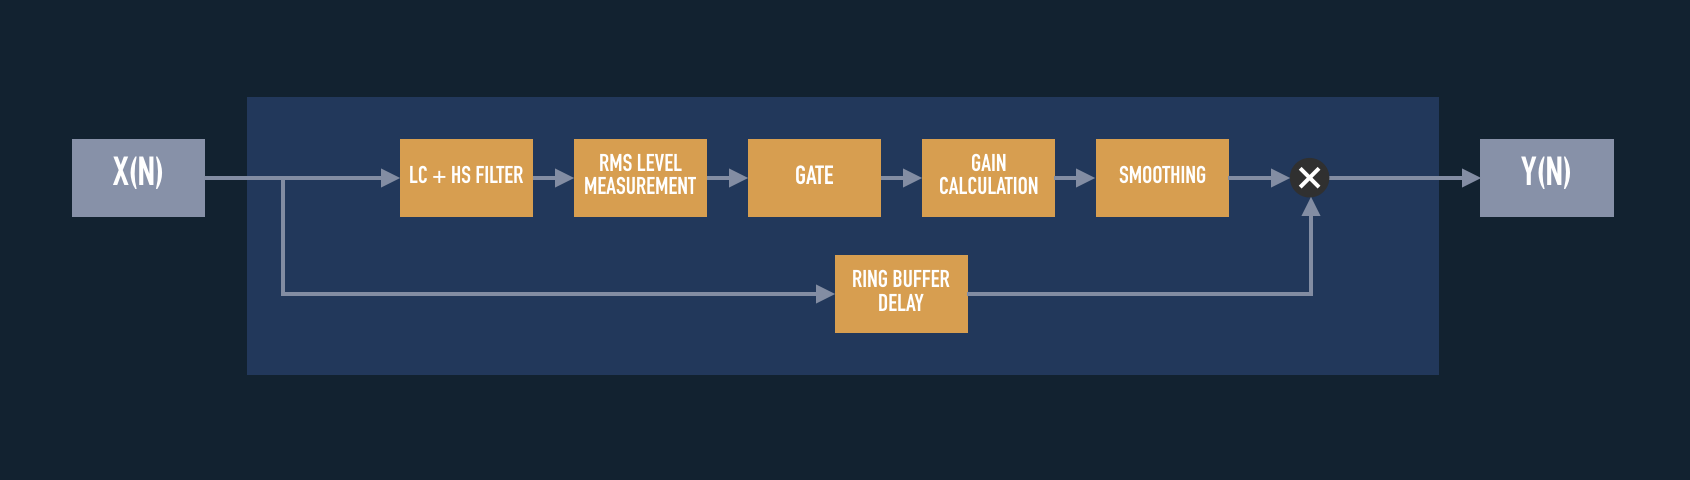
\includegraphics[width=\textwidth]{images/chain01}
\caption{Prototype processing chain}
\end{figure}

\section{Filter}

While gathering information on how to improve my idea of the plug-in I got interested in the ITU-R BS.1770-4 [FOOTNOTE pls] algorithm. It classifies an audio file for its humanly perceived loudness. The main use of this algorithm is found in television and music streaming services as they can keep the program loudness steady while switching content. As the human perception is also of interest for mixing a song, I examined how it was done. Due to a good documentation about how to implement the loudness algorithm I build a copy of it in python and decided which elements I would adopt in my plug-in. The first elements were the two filters. Like described above, their use is to mimic the human perception of sound pressure at different frequencies. The first filter is a low cut for the reason that human hearing is insensitive to low frequencies. The second filter is a high shelf and is ”used to account for the acoustic effects of the head” [wie zitiert man]. This imitation of the human hearing is greatly simplified but cost effective in terms of computation. The low cut filter has a cutoff frequency at 38 Hz, the high shelf around 1681 Hz. They are initialised at every plug-in startup in the JUCE method “prepareToPlay” with the current sample rate of the integrating DAW:\\

\lstset{language=C++}
\begin{lstlisting}[frame=single]
lowcut.setCoefficients(38.0, sampleRate, (1.0/2.0));
highshelf.setCoefficientsShelf(1681.0, sampleRate, 4.0);
\end{lstlisting}

The implementation is based on the biquad filter from the Book BLA (BLA NOTE auch im code).  I have chosen the second order biquad filter architecture as it is a very flexible and simple solution with just two samples delay. The calculation of filter coefficients is adopted as follows:

$f_c = $ cut-off frequency, $f_s = $ sampling frequency (rate), $K = tan(\pi f_{c}/f_{s})$,\\
$Q = $ factor for height of the resonance, $G = $ gain, $V_0 = 10^{G/20}$

\textbf{Lowcut:}\\
$b_0 = \frac{Q}{K^{2}Q+K+Q}$ \tab $b_1 = -\frac{2Q}{K^{2}Q+K+Q}$ \tab $b_2 = b_0$\\
$a_1 = \frac{2Q*(K^{2}-1)}{K^{2}Q+K+Q}$ \tab $a_2 = \frac{K^{2}Q-K+Q}{K^{2}Q+K+Q}$

\textbf{Highshelf:}\\
$b_0 = \frac{V_0+\sqrt{2V_0}K+K2}{1+\sqrt{2}K+K^2}$ \tab[0.4cm] $b_1 = -\frac{2(K^2-V_0)}{1+\sqrt{2}K+K^2}$ \tab $b_2 = \frac{V_0-\sqrt{2V_0}K+K2}{1+\sqrt{2}K+K^2}$\\
$a_1 = \frac{2(K^2-1)}{1+\sqrt{2}K+K^2}$ \tab $a_2 = \frac{1-\sqrt{2}K+K^2}{1+\sqrt{2}K+K^2}$\\

Hence the loudness algorithm uses second order filters (with two delay memories) it works like this:

Biquadfilter Bild

It is the same as my implementation in the Filter class:\\

\begin{lstlisting}[frame=single]
double AutoVocalCtrlFilter::process(double sample)
{
    const double mid = sample - a1 * z_1 - a2 * z_2;
    const double out = b0 * mid + b1 * z_1 + b2 * z_2;
    
    z_2 = z_1;
    z_1 = mid;
    
    return out;
}
\end{lstlisting}

Before implementing in C++ I testen my filter class in python. Therefor I send different signals with frequencies between 0 and 20000Hz through both filters and plotted the resulting amplitudes in a graph via pyplot(alter fußnoten verweis?). The current algorithm results in a descent graph (Fig. 3.2 NOCH ÄNDERN). To test the C++ version of the filter I compared the results of the same input with the previously tested python implementation.\\
The implementation is capable of many filter styles at different cutoff frequencies. For my plug-in it is used for the low cut and high shelf filter described above, which are simply processed one after the other on the current audio sample for each channel Wie VIELE AM ENDE??:\\
\begin{figure}
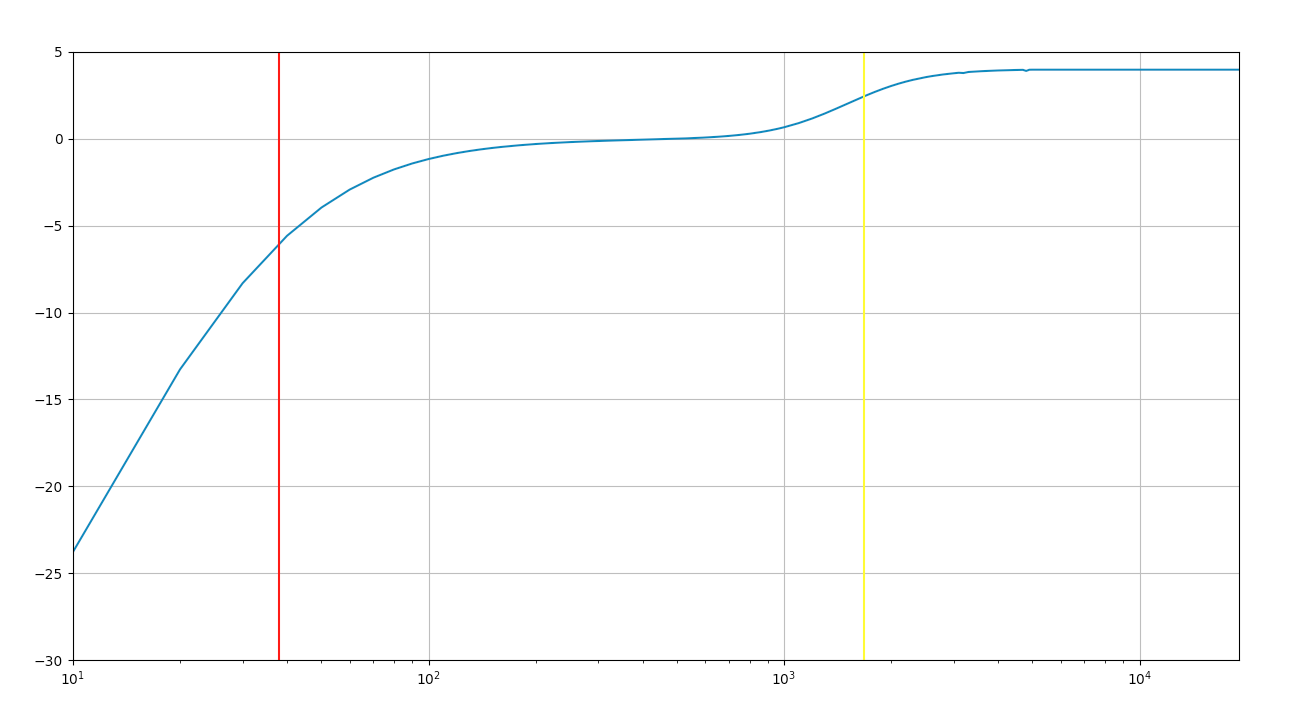
\includegraphics[width=\textwidth]{images/filter_test}
\caption{Plotted filter test}
\end{figure}

\begin{lstlisting}[frame=single]
double updateFilterSample(double sample, AutoVocalCtrlFilter hs,
AutoVocalCtrlFilter lc)
{
    return hs.process(lc.process(sample));
}
\end{lstlisting}

The updateFilterSample method returned the filtered samples for further processing.\\

\section{RMS}

To measure the level of the audio signal at the current position the plug-in calculates a root mean square (RMS) value of the last XX ms. This means it is calculating the root of the average from the squares of each sample in the set time window.\\
It uses RMS calculation because it is part of the imitation of human perception and because it has the necessary time to calculate an average value as it does not need to react fast. A human will (F. A. Everest, The Master Handbook of Acoustics, New York: McGraw-Hill, 2001.) not interpret a small impulse of a handful of samples as loud as a audio signal at the same level of longer duration.  For example “a 3-msec pulse must have a level about 15 dB higher to sound as loud as a 0.5-sec (500-msec) pulse”. This is also part of the BLABLA loudness standard. Additionally the “RMS is equal to the value of the direct current that would produce the same average power in a resistive load” [wikipdia].\\
The RMS implementation is based on the Book Digital Audio Signal Processing by Udo Zölzer (123) and can be performed in one line of code:\\

\begin{lstlisting}[frame=single]
double updateRMS2(double sample, double last, double co)
{
    return (1. - co) * last + co * (sample * sample);
}
\end{lstlisting}

The already filtered samples are used for this calculation and the result is written into the rms2 vector. The Co parameter is a time coefficient (see gleich) of small size. This parameter influences the weight on how much the current squared sample will inflict the quadratic mean. In normal RMS procedure the final result is the square root of the value the plugin results in. In this case we can skip the calulation because it will be converted into the logarithmic dB scale in the next step and a square just changes the value of one coefficient in this process. The final RMS value will only appear as logarithmic dB but save a little time.\\

\section{Time Coefficients}

The time coefficients are used for RMS calculation and to realise the compress and expand times (see later). They are determined with a formula by Udo Zölzer (quell):

$$1.f - \exp(-2.2*(1./currentSampleRate)/(ms/1000.))$$
$$=  1.f - \exp(-2.2*(1./currentSampleRate)/s)$$

Udo Zölzer decided to use the exponential function because it draws a natural decay. He determined -2.2 for the first part in the exponent by solving an equation system to achieve an attack time MATHE ta = t90 - t10. This means that when a calculation similar to the RMS calculation defined above uses such an time coefficient, its reaction on a input change will need the chosen amount of time to get from 10% of the final reaction to 90%. Illustrated in Fig.SIEHE UNTEN.
The second part in the exponent (1./currentSampleRate)/s) calculates the proportion of one sample to the amount of seconds of the MATH ta. This needs to be done because it will be used on every sample.

BILD MIT ATTACK ZEIT ODER RMS MITTEL DURCH IMPLUSE VERÄNDERUNG t90 und t10\\

\section{Gate}

The plug-in should operate while there are vocals and stop if there are none or just a soft decay. Else it would produce unwanted effects by amplifying noise. Additionally it would distort the applied gain for the actual vocals through strong gain increase at the gaps in-between.\\
To solve this potential problem the plug-in uses a gate. The gate checks for every sample if the sound pressure level is over a certain threshold. If not, it will be replaced by the current loudnessGoal. As the threshold and the loudnessGoal are set in dB, the first step in the gate is to convert the transferred sample ($rms^2$)  into the logarithmic scale. It uses $10.0 * std::log10(rms2 + 1e-10)$ instead of $20.0 * std::log10(rms + 1e-10)$ because the rms2 is squared. It adds MATH $+ 1e-10$ to head off the undefined $log10(0)$ case. After the conversion it gates the dB rms sample value at the dB threshold.\\
The threshold is defined as loudnessGoal - gainRange IST SO GEBLIEBEN?. Thereby it is still possible to use the whole gainRange for gain adaption and at the same time sort out the decay of the vocals. With this formula the threshold adjusts to the level of the vocals as the loudnessGoal is detected (see später).\\
When rms samples are not passing the gate and therefore being replaced by the loudnessGoal the plug-in adapts the gain to 0 (after a short period of time) because it has achieved its goal (see gain).\\

\section{Gain}

Now the most crucial part is happening: the calculation of the final gain value for the current sample.

\begin{lstlisting}[frame=single]
double updateGain(double sample, double lastGn)
{
    const double g = *loudnessGoal - sample;
    const double co = g < lastGn ? compressTCo:expandTCo;
    updateAutomation();
    return clipRange.clipValue((1 - co) * lastGn + co * g);
}
\end{lstlisting}

At first it computes the difference between the loudnessGoal and the current processed sample. The result is the gain factor that would be necessary to get it to the loudnessGoal (by multiplying in the linear number space).\\
Since the plug-in is designed to react on loudness differences for longer duration than for example compressors or expanders do, the gain adaption is smoothed over a proportionate amount of time. The smoothing is attained similar to the RMS calculation but uses different time coefficients.\\
The fitting time coefficient is chosen by comparing the calculated gain factor g with the gain that the function had returned for the precious sample. If g is smaller than the last gain (lastGn) the gain for the current sample will be smaller too. Therefore the dynamics of the input vocals will be compressed in relation to the last processed sample so it chooses the compressTCo time coefficient. The other way round when dynamics are expanded the expandTCo time coefficient is chosen. Different time coefficients for expanding and compressing dynamics are useful as amplifying a signal can be risky, while compressing it causes no trouble. For instance boosting a weak signal also boosts all the recorded unwanted noise. Additionally digital dynamics are limited and as the signal expands it risks to clip at the 0dB cap and produce distortion.\\

EXPAND VIELLEICGHT SCHWEIRIGES WORT DAFÜR WEIL SCHON BESETZT
vielleicht leise geht unter lautes sticht auffällig raus

After calculating the smoothed gain it gets clipped at the user chosen range up to +/- 10dB.
On one hand this ables the user to adjust the maximum variation of dynamics on the other hand it prevents the gain to increase up to problematically high values. This does not happen during normal use in an expected environment but can’t be completely ruled out due to possible unknown software errors or an unknown environment. As an error in the adapted gain does not only affect further calculation results but also the mixing engineer who is listening to an amplified signal, it is of special importance to avert wrong values (see LAST CAP OF PLUGIN).\\
When the gain is finally determined it will be converted back to the linear number space. Now it just needs to be multiplied with the current sample.\\

\section{Lookahead}

\begin{figure}[H]
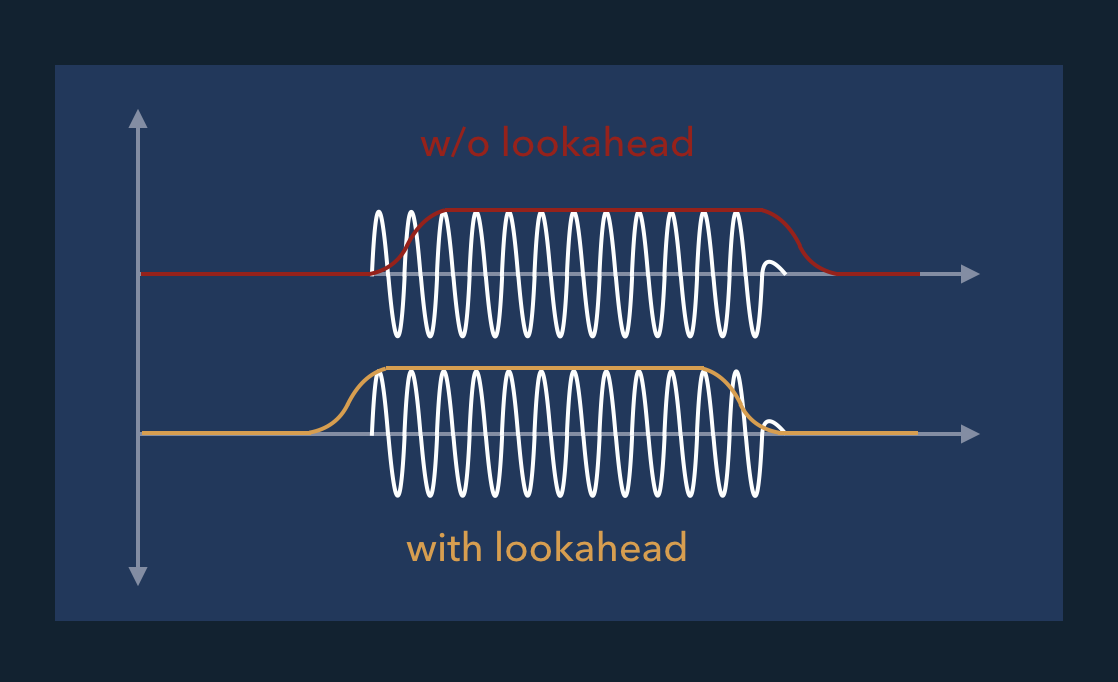
\includegraphics[width=\textwidth]{images/lookahead_w_o}
\caption{Gain adaption with and w/o lookahead}
\end{figure}

To achieve its goal the plug-in is designed to react slow and therefore needs some time adapt on a change in the average signal level. If it multiplies every sample with the gain value calculated form the same sample, the plug-in will be adjusted after the RMS has changed to the new average and the smoothed gain has slowly adapted. This will take some ms and consequently the first part of the alternate signal is not perfectly gained. While in particular this part introduces a new section in a song for example a chorus, it is desirable to have an adapted gain already at this point.\\
To compensate the adaption time I implemented a simple lookahead feature which allows the plug-in to calculate the gain for the current samples while looking at future samples.  This is realised by a ring buffer with two pointers at different locations. One write pointer to write the current sample transferred from the DAW into the buffer which is also used to determine the gain adaption and one read buffer ahead of it which is pointing on the sample that will be multiplied with the determined gain. To make this possible the gap between both pointers is as large as the set samples of the lookahead (converted from ms) and filled with zeros at the initialisation of the plug-in. In order to avoid that the whole plug-ins output is delayed I use the setLatencySamples()(see code besipel) method from JUCE to  communicate the resulting delay with the embedding DAW. Therefore a correct woking DAW will send the signal earlier to the plug-in and the output remains at the correct position despite the lookahead.\\
For the development I realised a fader in the UI to adjust the lookahead at runtime but in the final build the amount of samples is constant as I want the plug-in to be as simple to work with as possible. naja und weil ichja gewählt habe aus grund:

\begin{figure}[H]
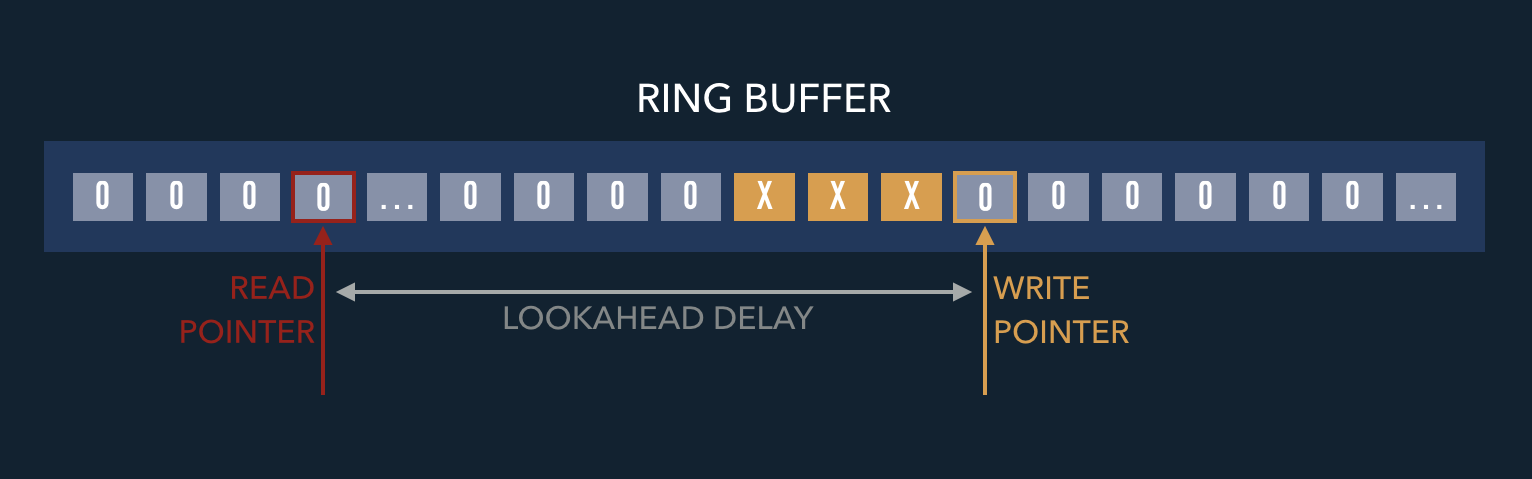
\includegraphics[width=\textwidth]{images/ring_buffer}
\caption{Initialized ring buffer with read and write pointers}
\end{figure}

vocals wichtig am Anfang erster push sollte nicht leiser gemacht sein weil vorher laut war oder andersrum
finale größe von delay sagen LOL
sollte nicht größer als ums sein oder
verweise zu den Bildern und code

\begin{lstlisting}[frame=single]
...
gain[channel] = updateGain(updateGate(rms2[channel], newGate),
gain[channel]);
double g = pow(10, gain[channel]/20);
delayData[dpw] = channelData[sample];
...
const double o = delayData[dpr] * g;
...
channelData[sample] = o;
...
if (++dpr >= delayBufferLength)
	dpr = 0;
if (++dpw >= delayBufferLength)
	dpw = 0;
...
\end{lstlisting}

\begin{lstlisting}[frame=single]
void AutoVocalCtrlAudioProcessor::updateDelay()
{
    int delayInSamples = msToSamples(*delayLength);
    delayReadPos = (int)(delayWritePos - delayInSamples
    + delayBufferLength) % delayBufferLength;
    setLatencySamples(delayInSamples);
}
\end{lstlisting}
\newpage\chapter{Improvements}
\label{chapter:improvements}

\section{Automation}

Using the study plug-in a mixing engineer will not have to draw gain automations manually. Nevertheless it can be useful to have an automation drawn by the plug-in. On one hand side it visualises the adapted gain curve better than the gain slider contained in the UI alone. On the other hand, it can save up calculation resources when the plug-in reads its own automation instead of processing the same vocal track in a repeated way. This is not necessary in simple mixing sessions but comes in handy when the mixed musical piece contains a great number of tracks with even more digital effects on each channel. Every digital effect increases the total amount of necessary CPU power. Often single tracks are bounced in place\footnote{all effects are rendered and combined with the actual signal to a new audio file} to avoid problems in performance. When the plug-in just reads an automation it is no considerable part of this problem even if there are multiple vocal tracks using this effect.\\
For those reasons the study plug-in was extended with this feature. In principle automations are supported by the JUCE framework and it can be very simple to implement a standard automation process. The normal case would be a user interacting with the UI and the plug-in communicating these changes to the DAW on write mode. On automation read mode the changes are send back to the plug-in during playback and it does its normal processing chain with changing parameters with the user drawn timing. The study plug-in was a special case which made it more difficult to realise the automation. In case of the study plug-in the write process of the automation should not be influenced by a user at intended use. Furthermore it should just receive and multiply the adapted gain from the drawn automation at read mode.\\
Like in the Waves plug-in a button was implemented at the UI to switch between read and write mode. Therefore the plug-in always knows if it needs to adapt the gain itself. The read mode implementation was performed quite fast as it just bypasses the regular calculations and multiplies the gain value set by the DAW with the current sample. The communication between DAW and plug-in works well on this part with the predefined parameter class from JUCE. The write mode produced more problems.\\
The plug-in adapts the gain value at write mode for every sample. When this would be communicated to the DAW like in normal automation process it has to draw at least 44100 adapted gain values each second. This easily overtaxes a DAW and is more accurate as it needs to be for a acceptable result. The DAW expects just a few changes per second for the automation as its normal use case (user modifies parameter at UI) would generate. It follows that the drawn automation had to be simplified.\\
At the first attempts automation changes were only communicated when the gain adaption changes its direction (compression/amplification) or when the difference to the last drawn automation point became crucial. Unfortunately this did not work as well. The output in the DAW would have been acceptable but at some spots it made incorrect jumps. These jumps occured in duration of at most 2 samples but they were still unwanted. Due to involvement of several devices in this process the real cause of the jumps could not be figured out. Different timings and positions for the communication to the DAW and also change of the parameter values were tested. During an long early testing phase no difference or worse results were achieved before an acceptable result was found:\\
The final solution sets a automation point every 80ms as long the gain changed about at least 0.1dB.
Therefore the gain adaption is constantly drawn in the automation curve but 12,5 instead of 41000 times a second or more. It does not set a new point when the gain is not adapting as this would be redundant. There are still jumps in the curve but this is acceptable as the jumps occur rarely and gain difference is about at most 0.1dB. Additionally these jumps are now located at correct positions without smoothing, which is not essential for such small amounts of adaption.\\

\begin{figure}[H]
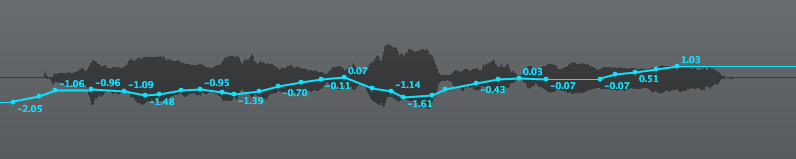
\includegraphics[width=\textwidth]{images/automation}
\caption{Automation written by the study plug-in into a DAW}
\end{figure}

\section{Adapting Loudness Goal}

The loudnessGoal parameter is not to understand as a gain controller. It is not designed to amplify the signal to a desired level. Instead, it should be adjusted to the actual loudness of the signal. In this way the plug-in can use its full range for changes on dynamics. For example when the loudnessGoal is set far below the signal level, the plug-in will stay at its minimal allowed gain value (initalized with -6dB) as long as it gets the high-level input. Even if it is at one end of the user defined dynamic range it will still operate in half (only negative/positive gain adaption) for most of the time. Therefore it is important to set the loudnessGoal correct. In best practice the plug-in will compress the incoming signal as much as amplifying it.\\
To simplify the selection of a fitting loudnessGoal for a user, a input meter was implemented next to the loudnessGoal slider and the current gain adaption. In this way it is easier to see if the current setting makes sense. However it still remains a problem as the perfect loudness goal possibly alters through a song. So it is difficult for a human to guess the average setting for the entire musical piece. Therefore some calculation based solutions were tested.\\
The first approach was determining a new loudnessGoal for every second. To achieve this the plug-in summed up all resulting gain values for each sample in this time period. Afterwards it calculated the average tendency (more positive or negative gain values). The offset was finally subtracted from the current loudnessGoal and the sum of the gain values got reseted.\\
Problematic with this approach was that the loudnessGoal adaption was one second to late if the signal level changed. In addition it made some advantages of the plug-in needless as it treated different parts of the vocals with different settings which results in some local benefits but leads to varying level through the whole track.\\
It follows that only analysing parts of the vocal track would not lead to a profitable result. Furthermore the plug-in should go through all critical parts of its input and therefore decide for the best suiting loudnessGoal. In conclusion a button was implemented accessible at the UI which switches the plug-in to loudnessGoal detection mode. During the time this mode is active the plug-in will not multiply the calculated gain with the signal but is still determining it, dissimilar to a regular bypass. In addition the plug-in re-adjusts its allowed gainRange for this period of time to the maximum (+/- 10dB). This is done to find a most accurate average loudness rate and it has no negativ consequences as it just endures as long as the detection mode is active. If you run the plug-in on detection mode through the full vocal track it calculates a decent loudnessGoal. To avoid the result being falsified by sections were no vocal signal is present, it only adapts on input with actual signal.\\
This is a task predestined to be done offline but due to the complexity of offline calculations in a plug-in operating in different DAWs the time was not enough to realise it in this thesis. For future work this would be a great opportunity to make use of the full ITU-R BS.1770-4 algorithm.\\
Although the loudnessGoal detection mode is probably the best current way to set the parameter, it is still allowed for a user to choose it him/herself due to own creative reasons.\\
When the loudnessGoal algorithmically adapts or is set to a new value on user terms the threshold of the plug-ins gate will change as well. Regardless of whether the average input is of small or great level the plug-in is therefore able to handle it with reasonable settings.\\

\section{Side Chain}

So far the plug-in works well on single audio tracks and reduces long term dynamics. This already lessens the work for a mixing engineer but the vocal level staying around the same amount over a whole musical piece is not necessary the wanted result. If the instrumental backtracks varies in its loudness it is desirable for the plug-in to do the same with its output gain. To do such a sing the plug-in requires additional information. Consequently a side chain input was added to its interface to realise this feature.\\
Side chains are not part of the standard I/O\footnote{I/O = input/output} layout of JUCE but supported since JUCE version 4.1. To realise another input, it was added in the BusesProperties() structure from the AudioProcessor class. As for the plug-in it is not necessary to have a side chain input, the supported bus layouts did not have to change. Therefore the embedding DAW is able to feed it with a signal but does not have to. For further testing in Logic Pro 9 the plug-in had to be revalidated for the DAW, before it accepted the new I/O layout. This was not necessary for previous algorithmic changes.\\
After implementing the new input the new information had to be used. To do this the plug-in reads the side chain buffer in its main processBlock() method. It needed information about the loudness of the backtrack (which should be fed into the side chain) to be able to determine a useful additional output gain. In process of detecting the loudness of the side chain input it is passing through the filter, RMS and gain calculations as the regular input signal does (see Fig. 5.2). This includes the transformation into logarithmic number space. Afterwards it is compared to the current loudnessGoal and the calculated difference is smoothed. Now the smoothed gain is transferred back to linear number space and it is multiplied with the gain of the parallel determination from the main input.\\
It is important for the side chain processing that it does not interfere with the main plug-in calculations. Especially the loudnessGoal must not be changed through this process. Otherwise it would corrupt its results in terms of dynamic range and make the loudnessGoal detection useless.\\
While testing in real use cases it seemed beneficial to add an additional output gain for the finally returned signal. This reduced the effort of matching vocal output level with the backtrack. It would be great if the plug-in could set the output gain itself depending on the side chain input, but as for different music styles and creative decisions there is not one right version of vocal to backtrack relation but a great number of reasonable possibilities. Nevertheless for future improvements of the plug-in this part can certainly be simplified in its user interaction.\\
The side chain feature remains an usable addition to the main plug-in but becomes no part of it as it is not automatically profitable in every use case. That is why there is button at the UI to toggle the 
side chain integration on and off. On further term this is useful as different DAWs will handle an undefined (when no input channel/bus is chosen) side chain input dissimilar. Logic Pro 9 sends for example an empty signal containing only zeros. This would effect the outcome of the plug-in when side chain integration is active as it would interpret the signal as a quiet backtrack. With the side chain activation button which is toggled off by default, there is no urgent need of a silence detection always running in the plug-ins side chain processing chain.\\
A remaining question for the side chain implementation were how to set the average time coefficients for RMS calculations and gain adaption (see 5.6). On one hand it should not react on small changes for example when a musician in the instrumental is just accentuating certain beats, on the other hand it needs to react fast enough to calculate an appropriate gain for the first sung words of a new song part with a different loudness level. Not negligible that it operates with the lookahead already realised for the plug-ins main use.\\
Additionally in the first approach it turned out to be a difficult problem for the side chain gain adaption to deal with instrumental breaks of longer duration (up to a full bar). While most of the instruments are pausing during those breaks the vocals should stay at the same level as it is often used to emphasize the remaining musicians. With the current implementation of side chain adaption instrumental breaks were causing a parallel slowly falling vocal level. Later with the implementation of the idle time (see 5.4) at gain adaption this behaviour could be avoided for the most part.\\

\begin{figure}[H]
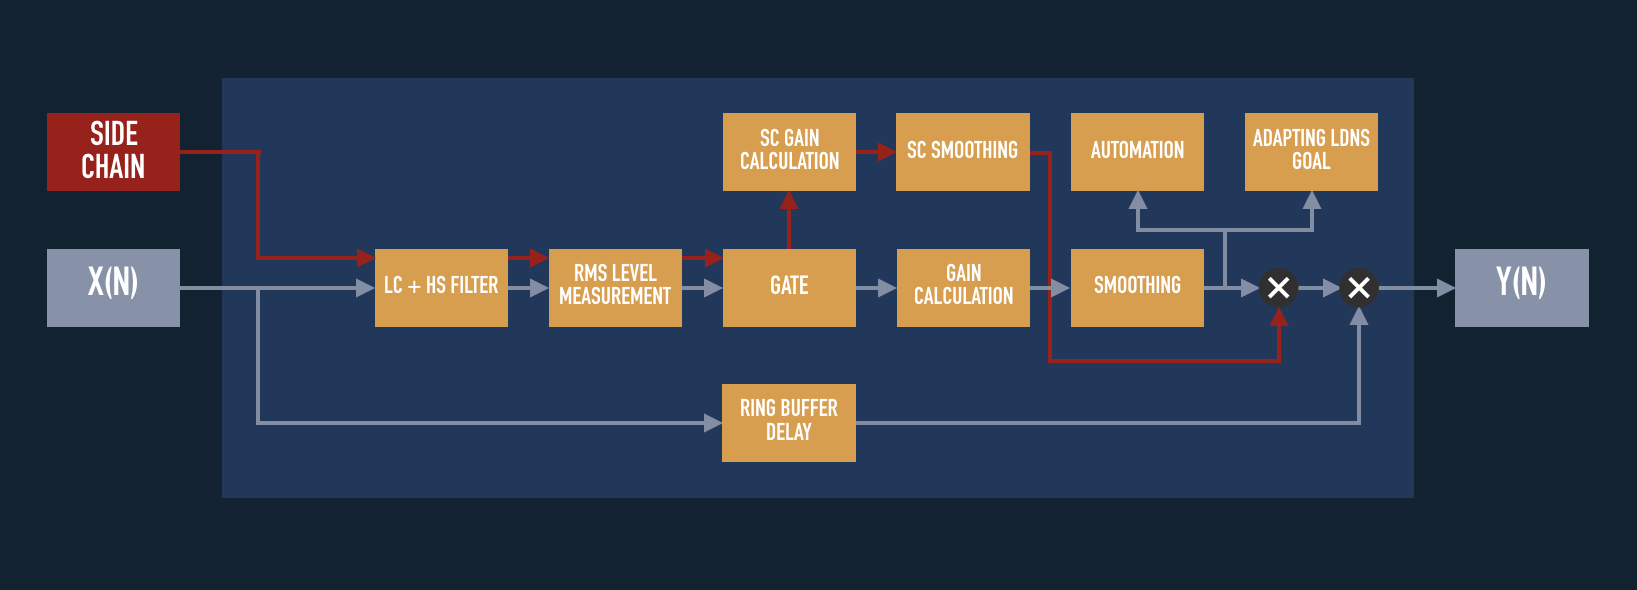
\includegraphics[width=\textwidth]{images/chain02}
\caption{Improved processing chain}
\end{figure}

\section{Idle Time}

During the comparison of the study plug-in and the “Vocal Rider” it emerged the idea of implementing a idle time before fading to 0dB gain for the study plug-in. The effect of such a idle time is that the plug-in will ignore short gaps between vocal signals. Therefore the plug-in does not change the adapted gain for example when a singer does a short rhythmic break in his/her vocals. So it will just use the actual vocals in the input for gain adaption similar to how a mixing engineer would do it. Due to a reasonable short duration of the idle time it is still able to adapt to 0dB gain for parts without singing. Following there will be no problematic danger of amplifying unwanted noise. The short period after a vocal signal and before a part of silence were the plug-in is still idle will not remain much longer than the vocal decay and is even shortened by the amount of lookahead delay.\\
At the first approach in implementing this feature the function of the gate was expanded. Every time the input was below the threshold, the current sample was replaced by the last one above for as long as the idle time was set. Due to the last sample above the threshold still being at proportional low level it did not work as planned. The subsequently gain adapting was consequently falling on even lower results than without the change at the gate because at idle time it got values near the lowest possible one which was just not set to the loudnessGoal by the gate. Maybe it could be fixed by replacing the samples at idle time with a RMS value from a sample further ahead, but this would require a additional memory for past samples and it seemed to complicated.\\
The current implementation is therefore based on the plan that the plug-in should detect at the gate if there are no vocals and then freeze the current gain at the following gain adaption. As the gain adaption is much slower due to compress/amplification time smoothing than the RMS averaging before the gate, it freezes the gain before it is able to adapt to the level change. For reasons of simplification everything was implemented in the updateGain method.\\

\begin{lstlisting}[frame=single]
double AutoVocalCtrlAudioProcessor::updateGain(double sample, 
double lastGn)
{
    if (sample != *loudnessGoal) {
        idleCount = 0;
    } else if (idleCount < maxIdleSamples) {
        idleCount++;
        return lastGn;
    }
...
}
\end{lstlisting}

It detects if the current level is below gate threshold by comparing the sample with the loudnessGoal. If the transferred RMS averaged sample is at the exact value of the loudnessGoal it can be assumed that the gate replaced its actual value. The rare case of a sample being randomly at exact the level of the loudnessGoal and therefore stop the gain adaption cant be eliminated in this simple implementation. Nevertheless this makes no a noticeable difference as it just stops the slow gain adaption for one single sample (max 1/44100 sec in expected use case). At the first sample differing from the loudnessGoal the idle timer is reset and the gain adaption continuous. When the maximum idle time is reached it has the same effect apart from resetting the idle time counter.\\
With the idle time working well in the main processing chain of the plug-in it was the next step to think about its advantages in terms of side chain integration. At this time there was still a problem with instrumental breaks and their unwanted impact on the calculated gain correction. Therefore a implementation of idle time similar to the already existing one for the main input was used. At the final side chain calculations it was implemented and adjusted the length of the maximum idle time with tests in a real mixing environment. The result with a reasonable set maximum was quite good as it severely reduced the gain drop during instrumental breaks as long as the side chain input level was adapted to the loudnessGoal. Consequently the UI was expanded with a pre gain slider for the side chain input which adds up before the comparison to the loudnessGoal. Controlling the input level of the side chain signal was possible before via a level controlled bus send but now the mixing engineer is able to do it all at one place while check the level meters for both signals right next to each other at the UI. As it was still difficult to adjust it correct for a whole song a self setting algorithm for the input gain was added to the already existing detection mode. As said before this would be significant better to do in an offline thread but works in real time for now.\\

\begin{figure}[H]
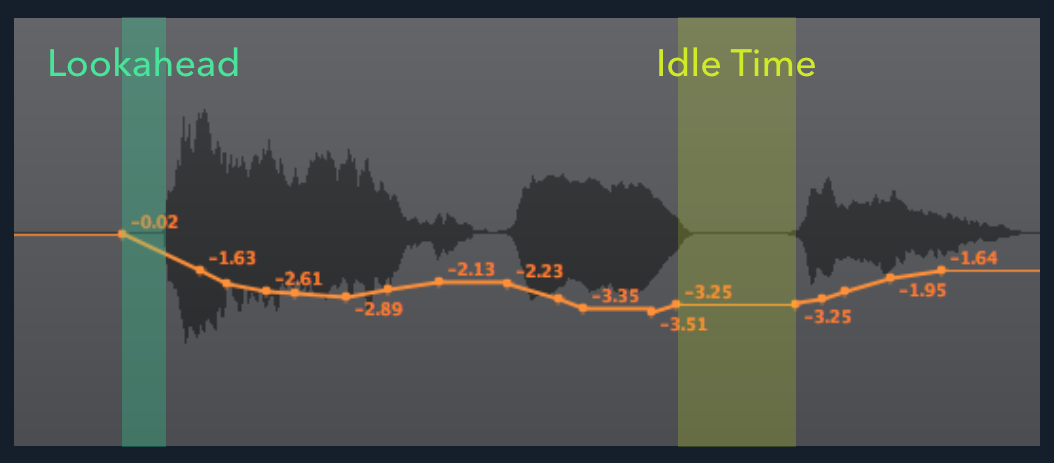
\includegraphics[width=0.8\textwidth]{images/automation2LookIdle}
	\centering
	\caption{Idle time and lookahead marked at automation written by the study plug-in}
\end{figure}

\section{Wet/Dry}

Many plug-in effects for DAWs have an additional slider to adjust the wet/dry ratio of their outcome. In these terms 100% “dry” is similar to the signal without the effect and 100% “wet” is a fully processed effect on the signal. This reduces the effort which would be necessary for sending the signal on a second track with the effect inserted to mix both tracks together in wanted proportions.\\
In consideration of the use of such a slider in the plug-in of this thesis, it seemed useful at first as it ables a user to set the intensity of dynamic compression. On the other hand this is already possible in a slightly different way with better outcome, by changing the current gainRange. In addition that this is feature has its main use in creative work, which is not the main objective of this plug-in, the final plug-in will not include a wet/dry slider for now. This decision was made with the intension of simplifying the UI to its foundation followed by the reduction of the settable parameters.\\

\section{Parameter Reduction}

As the plug-in slowly reaches its final state, it was necessary to transfer some settable parameters to fixed constants. In development it was useful to be able to change the important parameters while in runtime for example the compress and amplification times. Now it already emphasised which settings will  result in the best outcome. Small changes could be slightly better depending on the current circumstances but they are not required for a good result. Additionally with wrong application these parameters could create a poor result. Therefore and with the likely possibilities of a user not knowing what each of these parameters does, it seemed to be advantageous to hide those as constants, invisible at the UI.\\
This parameter reduction was applied to the lookahead delay, compress time, amplification time, RMS time, idle time, the side chain time constants and like already described, the gate. With the experience from testing the plug-in with many different settings in various circumstances the default choices for the parameters already got to reasonable values.\\
With a bad lookahead delay the gain adaption could happen to early or it has no noticeable effect. In the process of testing it commuted in at 60ms of delay as a good default value. For the parameter reduction it got set to 50ms as this resulted in the best outcome at additional test with special precision on the lookahead delay. A further test with a comparison of the drawn automation and the vocal signal waveform validated the new setting (see Fig. 5.1, 5.3).\\
The RMS averaging time shouldn’t be to long as this adds up on the total reaction time of the plug-in. On the other hand it needs a big enough time window to calculate a useful average. At the beginning of development it was set to 60ms. The comparison to the Waves “Vocal Rider” resulted in very small time windows (down to 8ms) for the averaging at this plug-in, to imitate the outcome. As this seemed a bit fast in consideration of previous experiences, it got into further tests with altering RMS time in collaboration with changing compress and amplification times. As result the RMS time is finally set to 30ms.\\
With the initialisation of two different attack times for compression and expansion it was manifested that the expansion time would be greater then the compression time. Still the final settings were not yet set. So again, the comparison to the “Vocal Rider” served as an inspiration. Though with a expansion time above two seconds it was not reacting fast enough to achieve the planned results, especially compared to the compression. As consequence the expansion time came down to 1500ms for the final build.\\
The compression time results from the comparison with the “Vocal Rider” were similar to a slow compressor and therefore still to fast to fit the idea of this thesis. As follows it had to be tested independently. This lastly resulted in a compression time of 600ms working out and, even though it was not planned, a slope of 1/3 at gain reduction. The reason for a additional slope were some vocal parts which got their level to low after compression. With a slope only at compression the gain adaption is balanced.\\
The idle time is set after considerations on the small gaps between phrases on vocal tracks. As it should be long enough to endure most of these gaps it is finally set to 500ms. A longer duration for the main functionality of the plug-in seemed unreasonable as it mainly extends the part after a vocal signal where the plug-in would just amplify noise.\\
For the side chain input the plug-in takes a idle time set to two seconds to be able to ignore instrumental breaks. With a shorter setting it still results in decreasing vocal level while those breaks are happening. Furthermore it uses the same RMS time like the main input and smoothes the resulting gain similar slow to the amplification time with a time coefficient adjusted to 1600ms.\\
The gate just adapts with the loudnessGoal like described in 5.2 and is not settable in the UI anymore.\\

\section{last CAP OF PLUG-IN}

\section{Design}


\newpage\chapter{Comparison}
\label{chapter:comparison}

After finishing the prototype of the plug-in, comparison of the main functionality with the equivalent from Waves was performed to find out how likely the results can get with fitting parameters at the prototype version of the implemented gain adaption and also to evaluate the flexibility of the study plug-in and to gather thoughts about how to set own parameters and constants later on.\\

\section{How}

It is expected that it would not be effective to try different picks for the parameters manually and compare the outcomes as there are at least several parameters which can be adjusted to result in a lot of combinations. Therefore, this task is transferred to the computer program.\\
The scipy.optimize package for Python deals with optimisation tasks for example the algorithmic minimisation of a problem according to the result of a self defined function (see chapter \ref{chapter:basics}.3).\\
Therefore a function to compare the resulting audio files after processed with the “Vocal Rider” and the study plug-in was developed. The resulting algorithm returns a value describing the deviation.\\
Through the optimisation process the parameter adjustments of the “Vocal Rider” differed between attempts but stayed constant in the process. The parameters of the study plug-in were changed continuously to achieve a preferably small deviation.\\

\section{Circumstances}

In order to let the optimisation algorithm amend different parts of the study plug-in, $L_{goal}$, RMS time, compress time, amplification time, gate threshold and lookahead delay are defined as variables. At start guessed values for each of the parameters are chosen and stored in an array which was altered through optimisation process and fed into the deviation function at every step of it.\\
For quantification of the deviation for the current parameter array the function sums up the squared difference between both resulting audio files for every sample. The result from the “Vocal Rider” was created in the DAW Pro Tools 11. The study implementation is called in the deviation function with the current parameter array.\\
When the optimisation search was done the outcome was fed into another function which displays the gain adaption from each plug-in in a collective graph. This gives a great overview of the result and remaining diversion of the implementations.\\

\section{Approaches}

Algorithmically the optimisation procedure tests small variations in the parameter array and watches the outcome. If the initial values were not set well, the differences calculated by the comparison function are small and the scipy.optimize.minimize algorithm did not know were to continue the search. With an unfavorable parameter set the gain curves are dissimilar and small variations might find a local minima in diversion but not the solution expected.\\
To obtain a good initial guess the scipy.optimize.brute method (see chapter\ref{chapter:basics}.3) was used. As just an approximation to the final solution was required large step sizes suiting the different ranges were set. Therefore the scipy.optimize.brute algorithm just had to deal with three to six possibilities per parameter.\\
The best initial values were fed into scipy.optimize.minimize. With good initialisation this method returned useful results meaning parameter arrays with likely outcome to the Waves plug-in. However the graphical representation of the 'Vocal Rider' gain adaption was not as expected: some gain values were jumping out of the line for single samples. After testing possible causes this could be explained by rounding errors of the DAW on export of audio files. While this error was unproblematic at most points in time, it became visible with values near zero. Such small values could easily be doubled or increased even further by the errors which consequently affected the calculation of the local gain. At first this was solved this with a gate for small samples at gain calculation. Afterwards it got fixed anyhow as the algorithm was changed to use RMS averages for displaying the graphical evaluation.\\

\begin{figure}[H]
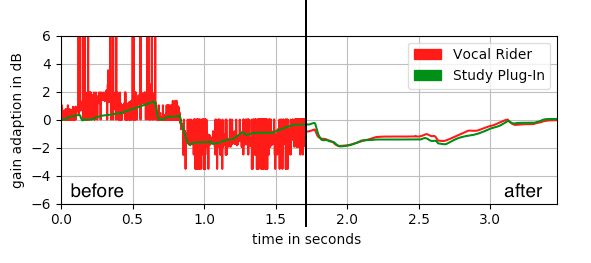
\includegraphics[width=\textwidth]{images/afterSmooth}
\caption{Optimisation result with (left) and w/o (right) rounding errrors}
\end{figure}

The behaviour of both plug-ins was compared by testing with optimised parameters on different vocal tracks in various length. The gain range of both plug-ins was set to +/- 6dB. The \textit{target} threshold of the “Vocal Rider” was adjusted to a reasonable value for all test files. The default and live component of the Vocal Rider were used. Additionally the plug-in from Waves wrote a gain automation and it read it through the export process for a further test file.\\

\section{Results}

The differences between the default “Vocal Rider” component, the live version and the self-automated were negligible. The automated plug-in provided in the same result as the default. It did not adapt for every sample but frequently after small consistent time steps, probably derivable from the communication between DAW and plug-in. The live version created no critical difference to the default - as it could be expected. It just added a potentiometer to adjust the noise gate for live performances. Therefore, in tests further described results will always relate to the default plug-in version.\\
The first analysis result was that the Waves plug-in is not using a lookahead and consequently the parameter optimisation always resulted in a lookahead value of 0ms. This was to expect for the live component but not necessary for its standard use, as today's DAWs can easily compensate the produced delay. Obviously it was not considered as important by the authors in contrast to the plug-in design in this study as explained in section 3.7.\\
The second analysis result was that the Waves plug-in does not start fading to 0dB gain immedietly when it detects no vocal signal but only after several milliseconds of idle time, in contrast to the study plug-in's prototype. This feature was assumed to enables the plug-in to ignore small gaps in the vocals when the singer is breathing or doing a rhythmic break where a smoothed gain reset to 0dB is not necessary and can even be counterproductive (as the gain adaption needs a few milliseconds). Therefore it resulted in the implementation of a similar function for the study plug-in as it was assumed to work even better in combination with a small lookahead (see chapter \ref{chapter:improvements}.4).\\
Despite the described obvious conceptual differences the optimisation algorithm was able to bring both plug-ins to quite close results in terms of the gain adaption. The “Vocal Rider” seems to need a short time (about one second) to adjust its behaviour. This presumption resulted from different tests where both plug-ins were operating quite similar except for the first second. As a consequence the compare function was improved by ignoring the first second of the result.\\
Initially the study plug-in was able to imitate a section of the “Vocal Rider”s gain adaption for test files of longer duration, but not to imitate the gain adaption for the whole signal. Therefore causes for this behaviour were evaluated taken into account that the amplification of the “Vocal Rider” with slow attack time results in greater gain alteration than the compression of it with very fast attack time. It seemed as if compression was attenuated while amplification was not. The weakened compression reminded of standard compressor behaviour. Therefore an additional ratio parameter was implemented for the Python test version of the plug-in. This parameter reduces the value of the calculated gain adaption before it is smoothed and applied. Subsequently the new parameter was added to the parameter array for the optimisation algorithm. Simultaneously, the lookahead optimisation was removed as it always resulted in 0ms. The extended optimisation validated the assumption described above and got both gain curves close together for the whole test files (see Fig. \ref{fresult}).\\
\begin{figure}
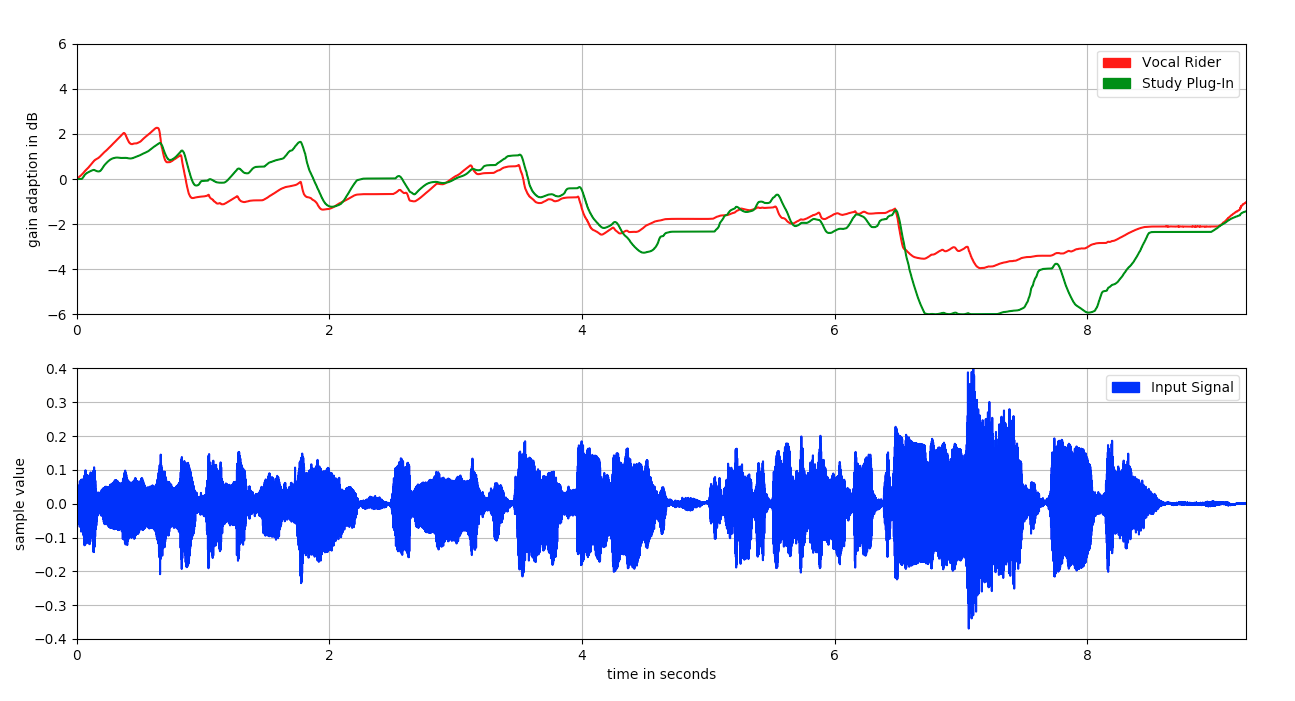
\includegraphics[width=\textwidth]{images/onlyParts}
\caption{Gain Reduction comparison with interim optimisation result}
\end{figure}
In conclusion it can be stated that the “Vocal Rider” does gain adaption on the decreasing part quite similar to a compressor but without any colouring of the altered signal and a small ratio\footnote{proportion between increment of input and output signal above the threshold}. The study plug-in was able to get a similar result with a compress time of barely 100ms and a additional gain factor of 2/3 (1/3 slope\footnote{slope $= 1 - 1/$ratio}) before smoothing. In terms of amplification of the input the plug-in by Waves takes a comparatively long time period. It takes a attack time of about 2,4s for the study plug-in to imitate its performance. The gate threshold-to-$L_{goal}$ relation of the study plug-in seems to fit the working method of the second test subject.\\
The comparison of the two plug-ins extended the main idea about some additional features and got some progress on the final set of the parameters to get to the main objective. Even though the results of the analysis of the “Vocal Rider” is not fitting the initial model of the study plug-in in all terms it still corroborated present work and leads to useful ideas.\\

\begin{figure}
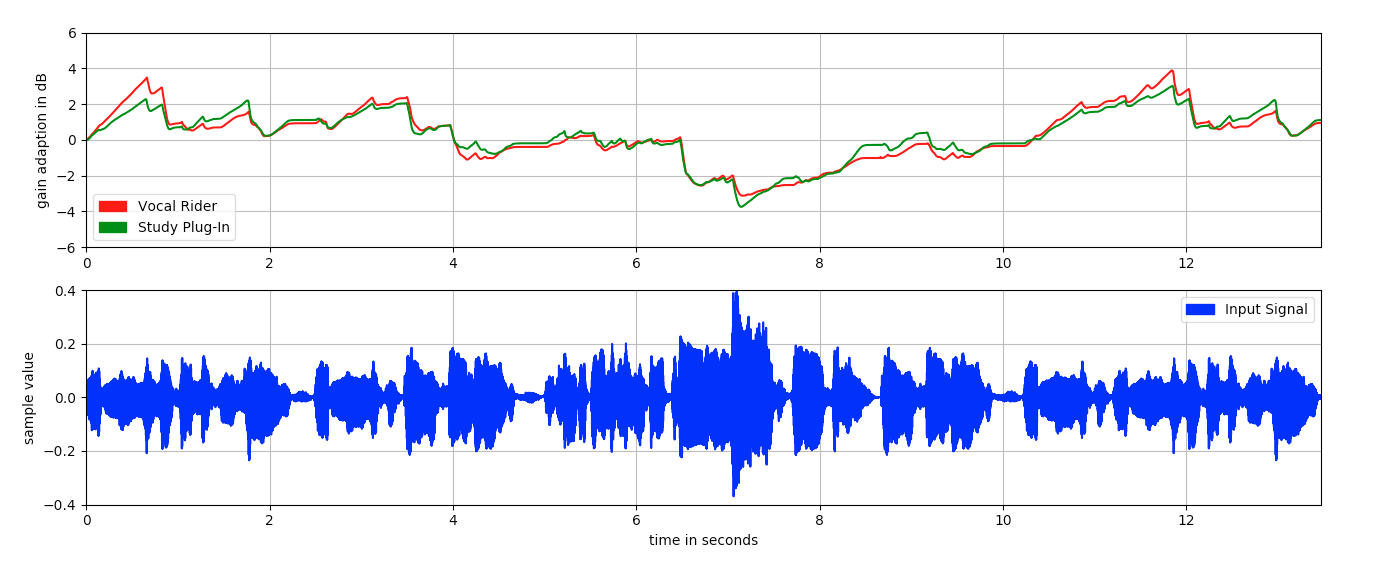
\includegraphics[width=\textwidth]{images/compareResult}
\caption{Gain Reduction comparison with final optimisation result}
\label{fresult}
\end{figure}
\newpage\chapter{Realization}
\label{chapter:realization}

\section{Parameter Reduction}

As the plug-in slowly reached its final state and the comparison to the 'Vocal Rider' was finished, it was necessary to transfer some settable parameters to fixed constants. In development it was useful to be able to change the important parameters while in runtime for example the compress and amplification times. Now it already emphasised which settings will result in the best outcome. Small changes could be slightly better depending on the current circumstances but they are not required for a good result. Additionally with wrong application these parameters could create a poor result. Therefore and with the likely possibilities of a user not knowing what each of these parameters does, it seemed to be advantageous to hide those as constants, invisible at the UI.\\
This parameter reduction was applied to the lookahead delay, compress time, amplification time, RMS time, idle time, the side chain time constants and like already described, the gate. With the experience from testing the plug-in with many different settings in various circumstances the default choices for the parameters already got to reasonable values.\\
With a bad lookahead delay the gain adaption could happen to early or it has no noticeable effect. In the process of testing it commuted in at 60ms of delay as a good default value. For the parameter reduction it got set to 50ms as this resulted in the best outcome at additional test with special precision on the lookahead delay. A further test with a comparison of the drawn automation and the vocal signal waveform validated the new setting (see Fig. \ref{auto2look}, \ref{auto}).\\
The RMS averaging time shouldn’t be to long as this adds up on the total reaction time of the plug-in. On the other hand it needs a big enough time window to calculate a useful average. At the beginning of development it was set to 60ms. The comparison to the Waves “Vocal Rider” resulted in very small time windows (down to 8ms) for the averaging at this plug-in, to imitate the outcome. As this seemed a bit fast in consideration of previous experiences, it got into further tests with altering RMS time in collaboration with changing compress and amplification times. As result the RMS time is finally set to 30ms.\\
With the initialisation of two different attack times for compression and expansion it was manifested that the expansion time would be greater then the compression time. Still the final settings were not yet set. So again, the comparison to the 'Vocal Rider' served as an inspiration. Though with a expansion time above two seconds it was not reacting fast enough to achieve the planned results, especially compared to the compression. As consequence the expansion time came down to 1500ms for the final build.\\
The compression time settings from the comparison with the 'Vocal Rider' were similar to a slow compressor and therefore still to fast to fit the idea of this study. As follows it had to be tested independently. This lastly resulted in a compression time of 600ms working out and, even though it was not planned, a slope of 1/3 at gain reduction. The reason for a additional slope were some vocal parts which got their level to low after compression. With a slope only at compression the gain adaption is balanced.\\
The idle time is set after considerations on the small gaps between phrases on vocal tracks. As it should be long enough to endure most of these gaps it is finally set to 500ms. A longer duration for the main functionality of the plug-in seemed unreasonable as it mainly extends the part after a vocal signal where the plug-in would just amplify noise.\\
For the side chain input the plug-in takes a idle time set to two seconds to be able to ignore instrumental breaks. With a shorter setting it still results in decreasing vocal level while those breaks are happening. Furthermore it uses the same RMS time like the main input and smoothes the resulting gain similar slow to the amplification time with a time coefficient adjusted to 1600ms.\\
The gate just adapts with $L_{goal}$ like described in \ref{chapter:improvements}.2 and is not settable in the UI.\\

\section{Python}

Development was not started with a final blueprint for the plug-in. Especially at the beginning several ideas on the basic algorithm, the gate or loudness detection were tested. In consequence the code had to be rearranged often. So Python came in handy as it focuses on code readability. In Python code there are fewer steps necessary to write the same program as for example in C++. Nevertheless, the plug-in was finally written in C++ (see below).\\
Furthermore, Python provides various packages which extend its scope by useful features. For example the matplotlib.pyplot\cite{MPlot} plotting framework enables to draw graphs of results. This was especially useful for testing on comparison results later on (see chapter \ref{chapter:comparison}) and the filter implementation.\\
To test the filter class and cutoff frequencies, different signals with frequencies between 0 and 20000Hz were send through both filters and the resulting amplitudes were plotted in a graph via pyplot. The final algorithm results in a descent graph (Fig. \ref{filterTest}). To test the C++ version of the filter subsequently the results of the same input with the previously tested Python implementation were compared.\\
The numpy\cite{numpy} package was essential for mathematical operations and the scipy\cite{scipy} tools were very useful in terms of audio handling and optimization (see chapter \ref{chapter:basics}.3). For this study Python version 3.6 was used.\\
Nevertheless Python was not the final choice for the plug-in as the C++ based JUCE framework offers a great predefined interface for audio plug-ins as well as the ability of fast processing due to the hardware-oriented C++ language. Speed of calculations can be crucial for real-time audio processing.\\
To make use of the scipy.optimize package at the comparison, the code of the plug-in's pototype was primarily transferred from C++ back to Python.\\

\section{JUCE Framework And C++}

JUCE is a cross-platform framework for audio applications based on C++. The main advantage is that it contains the functions needed for compiling to a VST\footnote{Virtual Studio Technology plug-in architectur provided by Steinberg} or AU\footnote{Audio Unit plug-in architectur provided by Apple} plug-in. Therefore, the main focus could stay on the algorithm of the plug-in during development. The JUCE audio plug-in template can be easily extended with a simple UI with sliders for the parameters of the algorithm. This is useful for testing the effects of individual parameters. JUCE covers much of the communication with the DAW. Mostly this was fitting to the study plan and for this reason only a few parts in which the plug-in had special needs had to be overwritten.\\
The input for a JUCE plug-in is transferred in seperate buffer blocks. Dependent on the current set of the buffer size the plug-in will receive a buffer block of a known amount of samples. This buffer block will be processed using the method processBlock(). Inside the method each of the previously described work steps (see chapter \ref{chapter:prototype}, \ref{chapter:improvements}) will be performed directly or by calling a responsible method. Subsequently the processed samples will be written back into the current buffer and the next buffer will be handled.\\
To set correct coefficients for the filters at possibly varying sample rate $f_s$, they are initialised at every plug-in startup in the JUCE method “prepareToPlay” with the current $f_s$ of the integrating DAW.\\
The lookahead delay is realised by a ring buffer with two pointers at different locations. One write pointer to write the current sample transferred from the DAW into the buffer which is also used to determine the gain adaption and one read buffer ahead of it which is pointing on the sample that will be multiplied with the determined gain (see Fig. \ref{RBuf}). To make this possible, the gap between both pointers is as large as the set samples of the lookahead (converted from ms) and filled with zeros at the initialisation of the plug-in.\\

\begin{lstlisting}[frame=single]
void AutoVocalCtrlAudioProcessor::updateDelay()
{
    int delayInSamples = msToSamples(*delayLength);
    delayReadPos = (int)(delayWritePos - delayInSamples
    + delayBufferLength) % delayBufferLength;
    setLatencySamples(delayInSamples);
}
\end{lstlisting}

When a pointer hits the end of the buffer it is set back to the start (see code example below) which leads to the imitation of a ring.\\

\begin{lstlisting}[frame=single]
delayData[dpw] = channelData[sample];
...
const double o = delayData[dpr] * g;
...
channelData[sample] = o;
...
if (++dpr >= delayBufferLength)
	dpr = 0;
if (++dpw >= delayBufferLength)
	dpw = 0;
\end{lstlisting}

In order to avoid that the whole plug-in's output is delayed the setLatencySamples() (see first code example) method from JUCE was used to communicate the resulting delay with the embedding DAW. Therefore a correct working DAW will send the signal earlier to the plug-in and the output remains at the correct position despite the lookahead.\\
For the development a fader in the UI was realised to adjust the lookahead at runtime, but in the final build the amount of samples is constant as the plug-in is designed to be as simple to work with as possible.\\

\begin{figure}[H]
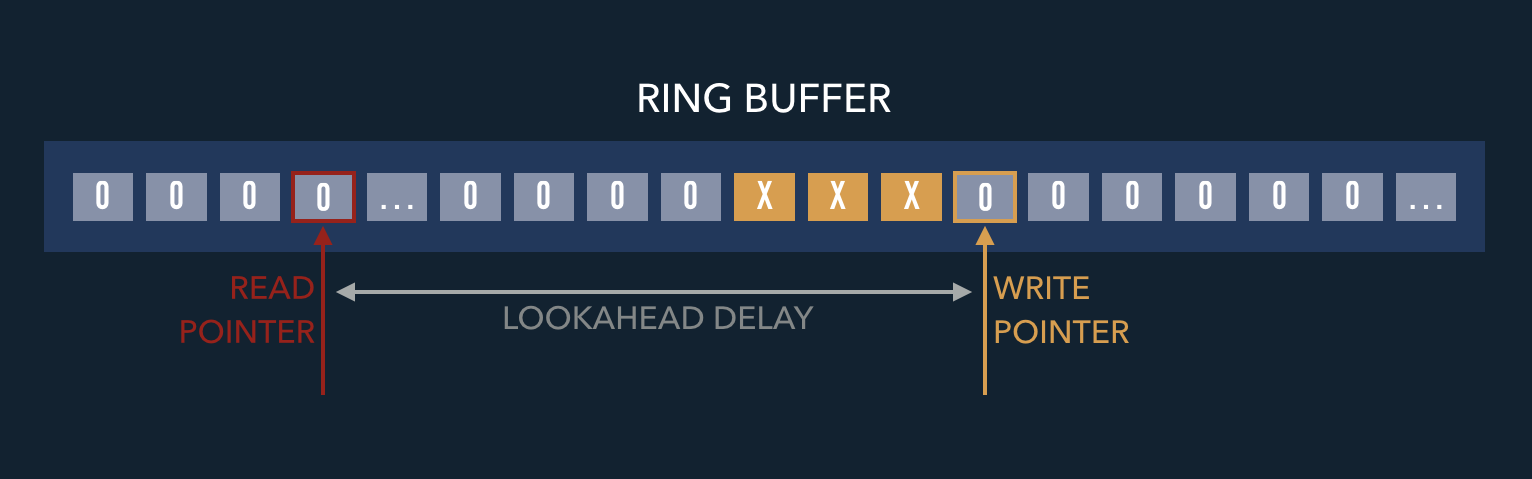
\includegraphics[width=\textwidth]{images/ring_buffer}
\caption{Initialized ring buffer with read and write pointers}
\label{RBuf}
\end{figure}

In principle the implementation of automations are supported by the JUCE framework as well and it can be very simple to implement a standard automation process. The normal case would be a user interacting with the UI and the plug-in communicating these changes to the DAW on write mode. On automation read mode the changes are send back to the plug-in during playback and it does its normal processing chain with changing parameters with the user drawn timing. The study plug-in was a special case which made it more difficult to realise the automation. In case of the study plug-in the write process of the automation should not be influenced by a user at intended use. Furthermore it should just receive and multiply the adapted gain from the drawn automation at read mode.\\
Like in the Waves plug-in a button was implemented at the UI to switch between read and write mode. Therefore the plug-in always knows if it needs to adapt the gain itself. The read mode implementation was performed quite fast as it just bypasses the regular calculations and multiplies the gain value set by the DAW with the current sample. The communication between DAW and plug-in works well on this part with the predefined parameter class from JUCE. The write mode produced more problems.\\
The plug-in adapts the gain value at write mode for every sample. When this would be communicated to the DAW like in normal automation process it has to draw at least 44100 adapted gain values each second. This easily overtaxes a DAW and is more accurate as it needs to be for a acceptable result. The DAW expects just a few changes per second for the automation as its normal use case (user modifies parameter at UI) would generate. It follows that the drawn automation had to be simplified.\\
At the first attempts automation changes were only communicated when the gain adaption changes its direction (compression/amplification) or when the difference to the last drawn automation point became crucial. With this procedure the output in the DAW would have been acceptable but at some spots it made incorrect jumps. These jumps occured in duration of at most 2 samples but they were still unwanted. Due to involvement of several devices in this process the real cause of the jumps could not be figured out. Different timings and positions for the communication to the DAW and also change of the parameter values were tested until the final solution was found (see chapter \ref{chapter:improvements}.1).\\
There are still jumps in the curve but this is acceptable as the jumps occur rarely and gain difference is about at most 0.1dB. Additionally these jumps are now located at correct positions without smoothing, which is not essential for such small amounts of adaption.\\

\begin{figure}[H]
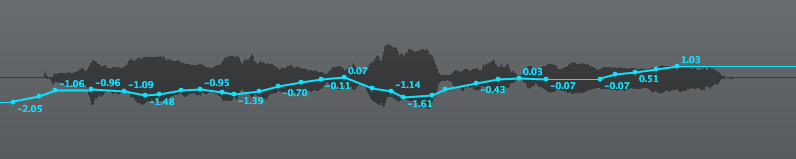
\includegraphics[width=\textwidth]{images/automation}
\caption{Automation written by the study plug-in into a DAW}
\label{auto}
\end{figure}

To simplify the selection of a fitting $L_{goal}$ for a user, a input meter was implemented close to the $L_{goal}$ slider and the current gain adaption. In this way it is easier to check whether the current setting makes sense.\\
With the $L_{goal}$ detection algorithm a button was implemented accessible at the UI which switches the plug-in to $L_{goal}$ detection mode.\\
Side chaining as implemented in chapter \ref{chapter:improvements}.3 is not part of the standard I/O\footnote{I/O = input/output} layout of JUCE but is supported since JUCE version 4.1. To realise another input, it was added in the BusesProperties() structure from the AudioProcessor class. As for the plug-in it is not necessary to have a side chain input, supported bus layouts had not to be changed. Therefore the embedding DAW is able to feed it with a signal but does not need to do so. For further testing in Logic Pro 9\footnote{Logic Pro 9 is DAW developed by Apple} the plug-in had to be revalidated for the DAW, before it accepted the new I/O layout. This was not necessary for previous algorithmic changes.\\
The side chain feature is a addition to the main plug-in but becomes no constant part of it as it is not automatically profitable in every use case. That is why a button is implemented at the UI to toggle side chain integration on and off. On further term this is useful as different DAWs will handle an undefined (when no input channel/bus is chosen) side chain input in a dissimilar way. For example will Logic Pro 9 send an empty signal containing only zero values. This would effect the outcome of the plug-in when side chain integration is active as it would interpret the signal as a quiet backtrack. With the side chain activation button toggled off by default, there is no urgent need of a silence detection always running in the plug-ins side chain processing chain.\\
As consequence of the idle time being added to the side chain feature the UI was expanded with a pre-gain slider for the side chain input which adds up before the comparison to $L_{goal}$. Controlling the input level of the side chain signal was possible before via a level-controlled bus\footnote{A Bus is a single path for multiple audio sources to be routed and processed.} send but now the mixing engineer is able to do it all at one place while check the level meters for both signals right next to each other at the UI. 

\subsection{Store Settings}

At startup the plug-in regularly initialises with settings that may fit some use cases but always have to be checked and adjusted properly for the current audio tracks. As a mixing engineer could start a mixing process on one day and finish it on another he may save and close the project and the used DAW for the night. Therefore the plug-in needs to get its latest settings saved or else it would initialise with the unchanged startup setting. This problem already effects the UI at runtime when it is closed and opened again. While the parameters for processing still stay correct in this case the UI could show wrong values at sliders which are not correctly refreshed.\\
To prevent this problem the getStateInformation() and setStateInformation() which will be called by the DAWs are filled with the necessary save commands.\\

\begin{lstlisting}[frame=single]
void AutoVocalCtrlAudioProcessor::setStateInformation (const 
void* data, int sizeInBytes)
{
    ScopedPointer<XmlElement> xmlState (getXmlFromBinary (data, 
    sizeInBytes));
    if (xmlState != nullptr)
    {
        if (xmlState->hasTagName ("AutoVocalCtrl"))
        {
            *sc = (bool) xmlState
            ->getBoolAttribute ("sc", false);
            *read = (bool) xmlState
            ->getBoolAttribute ("read", false);
           ...
            *loudnessGoal = (float) xmlState
            ->getDoubleAttribute ("loudnessGoal", -20.0);
            *gainRange = (float) xmlState
            ->getDoubleAttribute ("gainRange", 6.0);
            ...
        }
    }
    ...
}
\end{lstlisting}

The plug-in creates a new xml file with the values of all settable parameters in the getStateInformation() method and reads the xml file for parameter adjustment in the setStateInformation() method. Finally the setStateInformation() method notices the UI to refresh the according parameter sliders.\\
As DAWs are calling those methods at different timing but always at startup and before the shutdown of the plug-in or the UI, all user made adjustments are saved and regained at startup. Additional in this way the DAW will be able save presets for the plug-in which can be used in other mixing session for example as orientation for the parameter adjustment.\\

\subsection{UI Design}

The main focus of this study was the algorithm behind the plug-in. Nevertheless it was the intension that a user should be able to work with the plug-in without reading a manual. Therefore the JUCE dummy UI was refactored after parameter reduction.\\
The main problem of the previous UI was the lack of the possibility to differ between sliders for parameter adjustments and elements which were displaying inside information of the plug-in (see Fig. \ref{UIold}). Additionally the slider labels had not enough space to display in complete length similar to the slider value displays which could already confuse a user by their large number.\\

\begin{figure}[H]
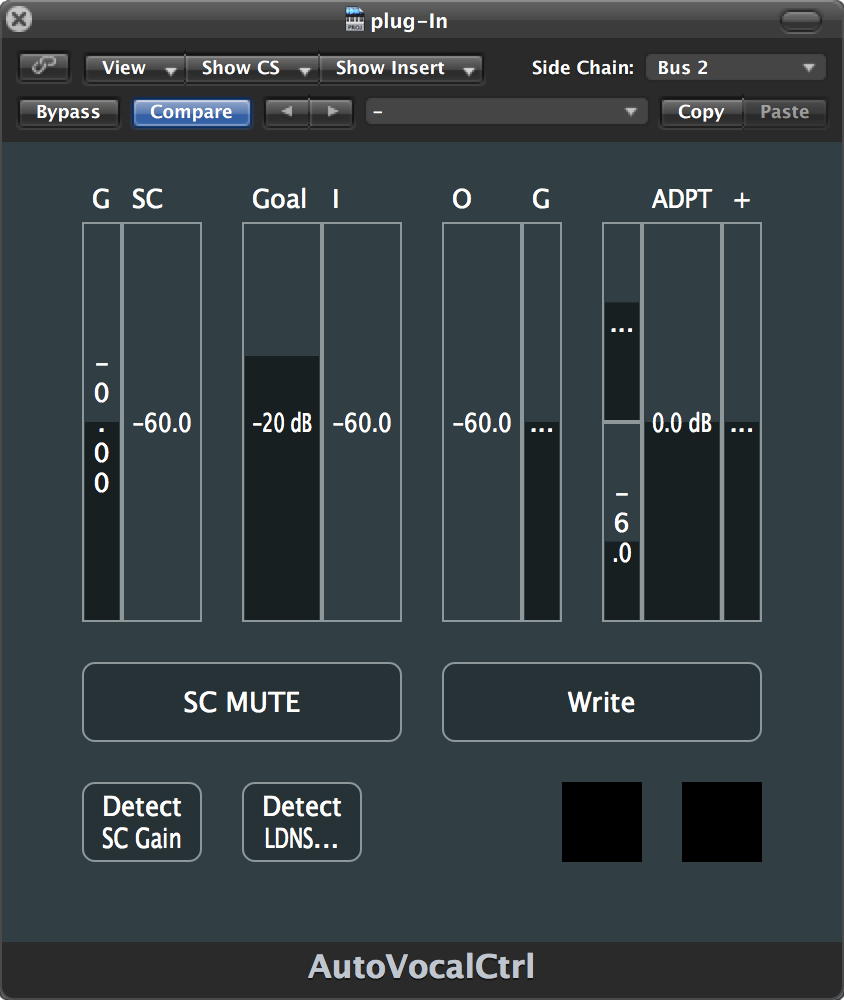
\includegraphics[width=0.5\textwidth]{images/designVorher}
	\centering
	\caption{UI after parameter reduction}
	\label{UIold}
\end{figure}

The main change in the UI re-design was the highlighting of usable elements. To set them apart from only informational parts, all the changeable components are coloured red. The colour is chosen as it strongly diverges from its complementary colour green which is the plug-in’s main colour (see Fig. \ref{UInew}). Additionally only the usable sliders and buttons got a coloured frame instead of the plain black outline of the pure metering components.\\

\begin{figure}[H]
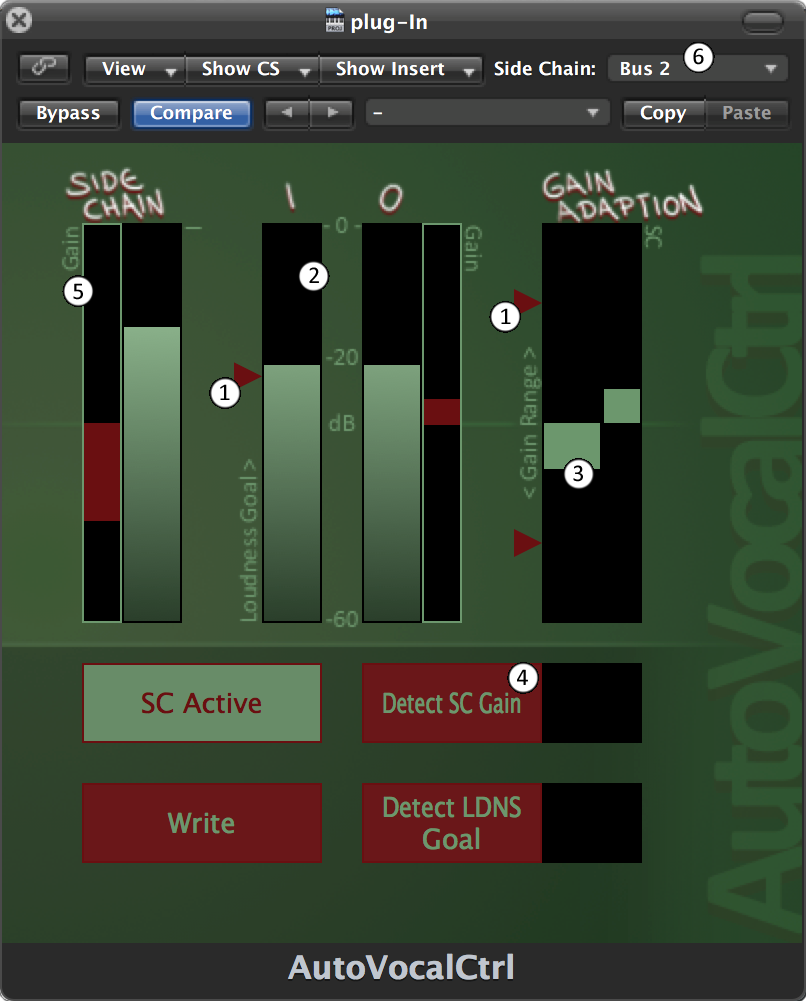
\includegraphics[width=0.5\textwidth]{images/designNeuNum}
	\centering
	\caption{Final UI in Logic Pro 9}
	\label{UInew}
\end{figure}

In the new design the gain range and loudness goal are set via red triangles (1) pointing on the corresponding level/gain meter. This was done to let the user to know the connection between these UI elements. $L_{goal}$ should be set in consideration of the input level meter (2) right next to it and the gain range is directly modifying the maximal and minimal values of the connected gain reduction meter (3).\\
The three meters which are displaying the I/O levels (input, side chain input, output) are next to each other and visualising their value with a rising bar where a colour gradient is applied to. Therefore the green tone of the bar is getting brighter with increasing signal level to support a fast assessment of the user.\\
All UI elements excluding the buttons are divided in different sections: The I (input), O (output), side chain and gain adaption section, containing the belonging components. To know which task the single components fulfil, they have a additional label, on the side which is not adjoining to another UI element.\\
When the Side Chain feature is disabled, the corresponding gain detection button (4) and the side chain input gain slider (5) become disabled too, as they would have no effect. This can be observed by the user as the red colour of these UI elements gets greyer and the slider loses its green frame which previously signalled a possible interaction. The components which are only for displaying information are disabled for user interaction by default.\\
For most of the slider elements it is not necessary for the user to know the exact value but to get a approximation and therefore a feeling about what is happening. Clear slider values often seduce users to adjust sliders to pretty numbers (e.g. rounding to 5 or repeated digits) instead of only observing the change of the outcome. As consequence most of the slider values are removed in the new design. A orientation for the input and output meters is still located next to them but in a light green like the element labels in order to not distract from the main information.\\
The side chain input (6) is chosen in the embedding DAW and therefore not to set in the plug-in’s UI.\\

\section{Test Environment}

The JUCE framework brings along two ways to run the plug-in. The fastest one is to build the plug-in as standalone which can be done directly from the IDE\footnote{integrated development environment}. The plug-in is starting immediately and the main input and output channels could be chosen. This is perfect for testing for small bug fixes or visual changes. The standalone procedure has its limitation in terms of e.g. a side chain input as it is not embedded in an surrounding DAW. But for this case JUCE has the Audio Plugin Host as solution. The Audio Plugin Host can host different plug-ins at the same time and visualises all inputs and outputs. It is enabling draw ing connections between those ports and the currently active audio interface of the operating computer. The advantage compared to a real DAW is that debugging output is provided through runtime.\\
Still it is necessary to test the plug-in in a real DAW for a realistic environment and to use all considered features, for instance writing an automation or comfortably feeding a real backtrack into the side chain input. Logic Pro 9 was used to run the study plug-in for the reason that it works with AU plug-ins which are per default supported by JUCE. Due to the custom UI it was still possible to change calculation parameters at runtime.\\
For tests in the DAW professional recorded audio tracks are needed additionally. For testing side chain adaption it was necessary to work with full musical compositions and not only to remain on vocal pieces. Therefore fitting multitrack projects from a online library\cite{MultiT} of free educational use were obtained (same as used in side chain evaluation, chapter \ref{chapter:evaluation}).\\
Before basic algorithmic tests were performed. Python was used because of its simplicity and helpful visual features. Therefore different approaches could be tested efficiently and visualised whether they have performed their task correctly.\\

\newpage\chapter{Evaluation of the Side Chain Feature}
\label{chapter:evaluation}

The plug-in was continuously improved during the testing period. One significant improvement was the side chain feature which will compensate for a whole further work step of the mixing engineer when it is functioning as intended. To proof the advantages of this feature a listening test was performed after the implementation. In the best case this could proof that there is no critical difference to a track volume automation additional to the main plug-in, drawn by a mixing engineer who knows about the level changes in the backtrack. At least it should verify the feature by demonstrating its advantages to the prototype in different circumstances.\\

\section{Test Conditions}

To receive results fitting the question about side chain advantages at the performed test, participants had to compare the backtrack/vocal level relation for audio files with the plug-in effecting the vocal gain with and without the side chain feature enabled. Additionally at every comparison there was a reference track where gain automations were drawn with oracle knowledge about the level change of the according backtrack. This track also had the plug-in inserted but without the side chain feature supporting. To establish the equivalence of the test scores an forth audio track with intensional divergent backtrack/vocal relation was added to perform as an anchor.\\
In the first 10 test sections 18 participants had to listen the reference track as aspired result and subsequently compare the backtrack/vocal level relation with four test items. The test items were mixes of the same song snippet but with varying gain adaption on the vocal tracks: the anchor with intensional divergent gain, a mix with the plug-in while the side chain feature was enabled, a mix altered by the plug-in without a side chain input and an unmodified copy of the reference. While comparing these test items with the first audio file declared as reference the participants did not know about the differences in the creation of the other four. The task was to rank the test items in their similarity of backtrack/vocal level relation to the reference on a percentage scale.\\
As the main plug-in is designed to push comprehensibility and clarity of the vocals in the mix, the question remained if an additional gain from the side chain feature could influence this in an unfavorable way. Consequently four additional test sections appended the procedure where comprehensibility and clarity where rated by the participants.\\
For the realisation of a valid test a important thing to do was picking usable song parts for the comparison. Therefore three different multitrack projects (see 2.3) were used as source for the audio snippets. As the benefit of the side chain feature is the adaption on backtrack level changes, at the beginning of all three songs the study plug-ins were initialised with settings to fit the local backtrack level. During this process loudnessGoal and side chain input-gain were set by the detection algorithm of the study plug-in. In the middle of the musical piece the backtrack level was changed due to a level automation. This was done in addition to the regular level changes of the backtrack to intensify the differences of the varying plug-in setting to be tested. The reference vocals with oracle knowledge got the same automations as the backtrack and where supplementary levelled to fit the backtrack at all the different song parts. The study plug-in with the side chain feature enabled had to adapt to the backtrack level changes itself while the same plug-in operated on the third vocal variation without the additional side chain informations. The level of the anchor was set manually in order to not resemble the reference track.\\
To have a wide range of circumstances tested for the plug-ins three to four different snippets were taken from each of the songs. These snippets are containing song parts before and after the backtrack level automation just like clips from the exact part where the level change is happening. Additionally the test was extended by snippets of song parts with vocals during instrumental breaks as these circumstances were especially difficult to handle at side chain feature development.\\
While the backtrack/vocal level relations were tested with all different kinds of snippets, the comprehensibility and clarity comparison was made with clips where the plug-in with the disabled side chain feature was adjusted in its output gain according to the current backtrack level to have a fair comparison. A single test was deviating from this scheme and therefore evaluated independently.\\
The test was realised in a HTML5 JavaScript browser application build with beaqlejs-0.2\cite{beaqleJS} using the MUSHRA test class. This framework already contained the necessary evaluation sliders and the functionality for the playback of the test items. To avoid confusion about comparison criteria the randomisation of test sections was disabled. Therefore the 10 backtrack/vocal level relation tests are followed by four comprehensibility and clarity tests. In order to receive independent results on each test the test items for evaluation are at randomised positions differing for each of the tests. During the tests the participants were listening to the audio clips on professional studio equipment in a quiet room for unadulterated results.\\
The results of test sessions were transferred into a table and subsequently evaluated.\\

\section{Vocal Level}

Due to the initialisation of the different set plug-ins for the test vocal tracks, the audio clips from the beginning of the songs have similar backtrack/vocal relations. Especially the oracle track and the plug-in without side chain have the same outcome at start. Despite the additional influence of the side chain algorithm the plug-in with the side chain feature enabled was ranked very close to the other two. The backtrack/vocal relation was judged not differing on average from the plug-in without side chain. As follows the side chain feature seems to have no unfavorable influence on the level outcome in comparison to a well gained (using the output gain to compensate the level gap between backtrack and vocals) plug-in without side chain.\\
At a backtrack level change the side chain feature has to adapt the level of the vocals and the plug-in without side chain will stay on the same output gain. As expected the vocal level results at backtrack level changes from the plug-in with side chain enabled were rated closer to the optimal reference. In average the side chain feature got the according test snippets rated 29\% closer to 100\% similarity with the reference as the plug-in without this feature. This average rating is very close to the rating of the reference copy. As consequence it is to conclude that the side chain feature leads to gain automations with similar results like a mixing engineer would draw. Additionally a advantage over the plug-in without a side chain input was observed.\\
The audio clips after backtrack level change, with the vocal level already adapted by the side chain feature, received ratings with even more advantage over the the plug-in without a side chain input. On average the side chain enabled plug-in was 35\% closer to the optimal result for each of those test files.\\
At instrumental breaks the ratings for the side chain adaption where about 5\% behind the total average but still better than the plug-in without side chain.\\
In total the similarity to the reference in terms of vocal/backtrack relation was rated 62\% for the plug-in without side chain. The side chain enabled plug-in got with an average value of 84\% very close to the copy of the optimal reference which was rated with 87\% similarity to itself on average.\\

\section{Comprehensibility}

Enhancing the comprehensibility and clarity of the vocals is an effect of the prototype plug-in in a professional mix as the vocals with lesser dynamics have fewer or no parts which are getting lost in a backtrack due to sectional lower loudness. Therefore it was important to test if the advanced comprehensibility and clarity of the vocals is decreased by the side chain feature which alters the outcome with an additional gain. As the relevant testing was done with audio snippets from the beginning of the song where the plug-in without side chain was initialised for the backtrack level, the question was if the additional side chain gain would have a bad effect or get similar results in comprehensibility and clarity.\\
In the according tests the participants had to rate comprehensibility and clarity also in comparison to a reference but with the exception that better clarity was rated with 100\% too. As result of the tests both main testimonials where rated for 90\% clarity in average. As conclusion the side chain feature does not seem to have a bad influence on clarity and comprehensibility as it got the same average test results as the plug-in without this feature.\\

\section{Test Results}

All in all the side chain feature proofed it self well in the accomplished testing. The clarity and comprehensibility of vocals does not seem to be effected in unfavorable manners by the enabled feature. In terms of backtrack level adaption it got the expected advantage, over the plug-in without this feature, verified (see table 6.1) and even rated close to the optimal drawn level automation with oracle knowledge.\\

\begin{table}[H]
\centering
	\begin{tabular}{ p{2cm} | p{3.5cm} | p{2cm} | p{2.5cm} | p{2cm} }
		& comprehensibility & \multicolumn{3}{ | c }{backtrack/vocal level relation} \\ \hline
		& before level change & before level change & during level change & after level change\\ \hline
		side chain advantage & 0\% & 0\% & 29\% & 35\% \\
	\end{tabular}
	\caption{Side chain advantages for different song parts}
\end{table}

In terms of the instrumental breaks the side chain feature could not continue its lead completely but still stays in advantage over the plug-in without these additional information. This is not the best result it could get but due to the initial difficulties it is still ranked as a success. While in the first versions of the side chain implementation it lowered the vocal level substantially during instrumental breaks, in the later versions there is no or only a very small level change observed under correct settings. Additionally, this is not an argument against using the side chain feature for those song parts, as in average it is still rated as advantage over the plug-in without the side chain feature, also by just considering instrumental breaks.\\
As the main backtrack level changes in the accomplished tests were artificially induced its results may not reflect for all possible circumstances. But as this supported the oracle knowledge of the reference track and made differences for the participants' ability to hear more clearly it seemed to be a good choice to do so. Additionally it is questioned whether every participant would be able to hear the differences if they had not been artificially induced differing enough.\\
The test results could be corroborated with additional participants but the 18 which had done the testing already revealed a plausible trend (see table 6.2).\\

\begin{table}[H]
\centering
	\begin{tabular}{ p{4cm} | c | c | p{4cm} }
		& plug-in & plug-in + sc & plug-in + oracle gain (copy of reference) \\ \hline
		similarity to reference on average & 68\% & 86\% & 89\% \\
	\end{tabular}
	\caption{Similarity to reference of test candidates}
\end{table}

Thereby it was observed that the side chain feature got near the optimal result and in any case validated its advantages over a plug-in without this feature. It was ranked better than its direct adversary in most of the cases (see Fig. 6.1).\\
As conclusion it seems to work properly and has legitimacy to be a part of the final product.\\

\begin{figure}[H]
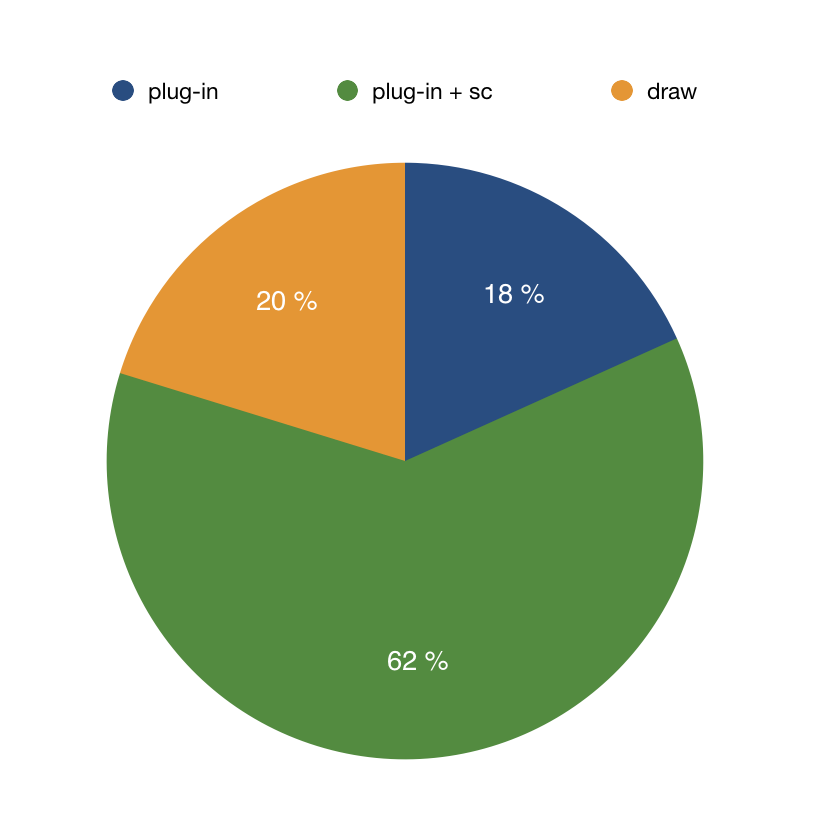
\includegraphics[width=0.55\textwidth]{images/betterRating}
\centering
\caption{Plug-in setting with better rating (all tests)}
\end{figure}

\newpage\chapter{Conclusion}
\label{chapter:conclusion}

The realisation of the objective could be achieved with a satisfactory result. During the process of development the JUCE Framework emphasises as a good choice by supporting with basic but solid functionality for an audio plug-in which would have been very time-consuming to build up from scratch.\\
With the first prototype version it was already possible to obtain favourable results (reasonable parameter settings implied). Nevertheless it still had some unfavorable problems and unfinished design decisions. The comparison to “Vocal Rider” approved the functionality of the prototype but also pointed out the differences between the two approaches of the plug-ins. Despite the differences the comparison resulted in ideas for further improvements of the study plug-in.\\
In retrospective view quite a lot improvements enhanced the early prototype. The additions with most influence on the plug-ins performance where the extra idle time for ignoring small breathing or rhythmic gaps between vocal signals, the ability to draw gain automations into the DAW, the side chain feature and the automatic detection of parameters.\\
The side chain feature validated its use in the according hearing test where its advantages for the plug-in where observable as well as the outcome of a plug-in with this feature enabled getting quite close to the optimal reference (which performed the gain adaption with oracle knowledge).\\

\section{Future Improvements}

The study plug-in meets the requirement of the objective but it could still be improved.\\
For example, parameter detection is an optional feature which could be useful to set the plug-in correctly, especially at first interactions of a user but as described in the corresponding chapter \ref{chapter:improvements}.2 and \ref{chapter:improvements}.3, it is only able to calculate ‘online’ during playback of the song. An offline calculation is not implemented yet which would be significantly faster. As one purpose of the plug-in is to save time for the mixing engineer, it would be great to enhance the feature with offline calculations in future development. When the offline calculation is possible it would be able to measure the perceived signal level by using the loudness algorithm\cite{ITUalgo} which may improve the plug-in’s outcome.\\
An other option of a reasonable future improvement would be to extend its scope of application. Currently it is designed to work with vocal signals but other recordings may show similar problems e.g. recordings of the bass guitar. Therefore it would be useful to have the opportunity to chose between different presets for the main constants of the plug-in’s calculation, fitting the different signals.\\
Additional to possible algorithmic improvements the plug-in could be improved by further testing for increased stability and correctness of the results.\\

\section{Conclusion}

A plug-in for decreasement of long term dynamics was developed. During the work on this study the plug-in’s prototype frequently changes and additional improvements in terms of features, algorithms and parameters were included.\\
It certainly might get further improvements in different parts but in final conclusion the study resulted in a plug-in mature enough to fulfil its intended task in daily production, and even some features more.\\




\finish